
% \documentclass[10pt,journal,cspaper,compsoc]{IEEEtran}
\documentclass[10pt,journal]{IEEEtran}

%
\ifCLASSOPTIONcompsoc
  % IEEE Computer Society needs nocompress option
  % requires cite.sty v4.0 or later (November 2003)
  % \usepackage[nocompress]{cite}
\else
  % normal IEEE
  % \usepackage{cite}
\fi

% *** GRAPHICS RELATED PACKAGES ***
%
\ifCLASSINFOpdf
  % \usepackage[pdftex]{graphicx}
  % declare the path(s) where your graphic files are
  % \graphicspath{{../pdf/}{../jpeg/}}
  % and their extensions so you won't have to specify these with
  % every instance of \includegraphics
  % \DeclareGraphicsExtensions{.pdf,.jpeg,.png}
\else
  % or other class option (dvipsone, dvipdf, if not using dvips). graphicx
  % will default to the driver specified in the system graphics.cfg if no
  % driver is specified.
  % \usepackage[dvips]{graphicx}
  % declare the path(s) where your graphic files are
  % \graphicspath{{../eps/}}
  % and their extensions so you won't have to specify these with
  % every instance of \includegraphics
  % \DeclareGraphicsExtensions{.png}
\fi
% graphicx was written by David Carlisle and Sebastian Rahtz. It is
% required if you want graphics, photos, etc. graphicx.sty is already
% installed on most LaTeX systems. The latest version and documentation can
% be obtained at:
% http://www.ctan.org/tex-archive/macros/latex/required/graphics/
% Another good source of documentation is "Using Imported Graphics in
% LaTeX2e" by Keith Reckdahl which can be found as epslatex.ps or
% epslatex.pdf at: http://www.ctan.org/tex-archive/info/
%
% latex, and pdflatex in dvi mode, support graphics in encapsulated
% postscript (.png) format. pdflatex in pdf mode supports graphics
% in .pdf, .jpeg, .png and .mps (metapost) formats. Users should ensure
% that all non-photo figures use a vector format (.png, .pdf, .mps) and
% not a bitmapped formats (.jpeg, .png). IEEE frowns on bitmapped formats
% which can result in "jaggedy"/blurry rendering of lines and letters as
% well as large increases in file sizes.
%
% You can find documentation about the pdfTeX application at:
% http://www.tug.org/applications/pdftex



% correct bad hyphenation here
\hyphenation{op-tical net-works semi-conduc-tor}

\usepackage{listings}
\usepackage[table]{xcolor}
\usepackage{graphicx}
\usepackage{amsmath}
\usepackage{amssymb}
\usepackage{color}
\usepackage{epsfig}
\usepackage{tabularx}
\usepackage{ctable}
\usepackage{multirow}
\usepackage{subfigure}
\usepackage{mathrsfs}
\usepackage{mathtools}
\usepackage{hyperref}
\usepackage{pbox}
\usepackage{epstopdf}
\usepackage{sci}

\newcommand{\Songfan}[1]{\textcolor{red}{#1}}

%\newcommand{\argmin}{\arg\!\min}
%\newcommand{\argmax}{\arg\!\max}

\begin{document}
%
% paper title
% can use linebreaks \\ within to get better formatting as desired
\title{A Dense Flow-based Framework for Real-time Object Registration under Compound Motion}
%Understanding Consumer Preference for Advertisement\\from Facial Expression}
%
%
% author names and IEEE memberships
% note positions of commas and nonbreaking spaces ( ~ ) LaTeX will not break
% a structure at a ~ so this keeps an author's name from being broken across
% two lines.
% use \thanks{} to gain access to the first footnote area
% a separate \thanks must be used for each paragraph as LaTeX2e's \thanks
% was not built to handle multiple paragraphs
%
%
%\IEEEcompsocitemizethanks is a special \thanks that produces the bulleted
% lists the Computer Society journals use for "first footnote" author
% affiliations. Use \IEEEcompsocthanksitem which works much like \item
% for each affiliation group. When not in compsoc mode,
% \IEEEcompsocitemizethanks becomes like \thanks and
% \IEEEcompsocthanksitem becomes a line break with idention. This
% facilitates dual compilation, although admittedly the differences in the
% desired content of \author between the different types of papers makes a
% one-size-fits-all approach a daunting prospect. For instance, compsoc
% journal papers have the author affiliations above the "Manuscript
% received ..."  text while in non-compsoc journals this is reversed. Sigh.

\author{Songfan~Yang,~\IEEEmembership{Member,~IEEE,}
				Le~An,~\IEEEmembership{Member,~IEEE,}
				Yiguang~Liu,
				Mingyang~Li,
        Ninad~Thakoor,~\IEEEmembership{Member,~IEEE,}
        and~Bir~Bhanu,~\IEEEmembership{Fellow,~IEEE}% <-this % stops a space
\IEEEcompsocitemizethanks{\IEEEcompsocthanksitem Acknowledgment: \IEEEcompsocthanksitem \protect\\ S.~Yang is with the College of Electronics and Information Engineering at Sichuan University, Chengdu, China 610064. E-mail: syang@scu.edu.cn \protect\\
L.~An is with University of North Carolina at Chapel Hill, Chapel
Hill, NC 27599 USA. E-mail: lan004@ucr.edu \protect\\
Y.~Liu is with the School of Computer Science at Sichuan University. E-mail: liuyg@scu.edu.cn \protect\\
M.~Li is with Google Inc., Mountain View, CA, 94043 USA. Email: mingyangli009@gmail.com \protect\\
N.~Thakoor,~and~B.~Bhanu are with the Center for Research in Intelligent Systems, University of California, Riverside, CA 92521 USA.\protect\\
E-mail: \{nthakoor,~bhanu\}@ee.ucr.edu}% <-this % stops a space
\thanks{}}

% note the % following the last \IEEEmembership and also \thanks -
% these prevent an unwanted space from occurring between the last author name
% and the end of the author line. i.e., if you had this:
%
% \author{....lastname \thanks{...} \thanks{...} }
%                     ^------------^------------^----Do not want these spaces!
%
% a space would be appended to the last name and could cause every name on that
% line to be shifted left slightly. This is one of those "LaTeX things". For
% instance, "\textbf{A} \textbf{B}" will typeset as "A B" not "AB". To get
% "AB" then you have to do: "\textbf{A}\textbf{B}"
% \thanks is no different in this regard, so shield the last } of each \thanks
% that ends a line with a % and do not let a space in before the next \thanks.
% Spaces after \IEEEmembership other than the last one are OK (and needed) as
% you are supposed to have spaces between the names. For what it is worth,
% this is a minor point as most people would not even notice if the said evil
% space somehow managed to creep in.



% The paper headers
\markboth{IEEE Transactions on Cybernetics}%
{Shell \MakeLowercase{\textit{et al.}}: Bare Demo of
IEEEtran.cls for Computer Society Journals}
% The only time the second header will appear is for the odd numbered pages
% after the title page when using the twoside option.
%
% *** Note that you probably will NOT want to include the author's ***
% *** name in the headers of peer review papers.                   ***
% You can use \ifCLASSOPTIONpeerreview for conditional compilation here if
% you desire.


% for Computer Society papers, we must declare the abstract and index terms
% PRIOR to the title within the \IEEEcompsoctitleabstractindextext IEEEtran
% command as these need to go into the title area created by \maketitle.
\IEEEcompsoctitleabstractindextext{%
\begin{abstract}

A moving object often has elastic and deformable surfaces (\textit{e.g.}, a human head). Tracking and measuring surface deformation while the object itself is also moving is a challenging, yet important problem in many video analysis tasks. For example, video-based facial expression recognition requires tracking non-rigid motions of facial features without being affected by any rigid motions of the head. In this paper, we present a generic video alignment framework to extract and characterize surface deformations accompanied by rigid-body motions with respect to a fixed reference (a canonical form). We propose a generic model for object alignment in a Bayesian  framework, and rigorously show that a special case of the model results in a SIFT flow and optical flow based least-square problem. We demonstrate that dynamic programming can be used to speed up the computation of our algorithm. The proposed algorithm is evaluated on three applications, including the analysis of subtle facial muscle dynamics in spontaneous expressions, face image super-resolution, and generic object registration. Experimental results, in terms of both qualitative and quantitative measures, demonstrate the efficacy of the proposed algorithm, which can be executed in real time.


\end{abstract}
% IEEEtran.cls defaults to using nonbold math in the Abstract.
% This preserves the distinction between vectors and scalars. However,
% if the journal you are submitting to favors bold math in the abstract,
% then you can use LaTeX's standard command \boldmath at the very start
% of the abstract to achieve this. Many IEEE journals frown on math
% in the abstract anyway. In particular, the Computer Society does
% not want either math or citations to appear in the abstract.

% Note that keywords are not normally used for peer review papers.
\begin{keywords}
Object registration, spontaneous facial expression, SIFT flow, optical flow, super-resolution
\end{keywords}}


% make the title area
\maketitle


% To allow for easy dual compilation without having to reenter the
% abstract/keywords data, the \IEEEcompsoctitleabstractindextext text will
% not be used in maketitle, but will appear (i.e., to be "transported")
% here as \IEEEdisplaynotcompsoctitleabstractindextext when compsoc mode
% is not selected <OR> if conference mode is selected - because compsoc
% conference papers position the abstract like regular (non-compsoc)
% papers do!
\IEEEdisplaynotcompsoctitleabstractindextext
% \IEEEdisplaynotcompsoctitleabstractindextext has no effect when using
% compsoc under a non-conference mode.


% For peer review papers, you can put extra information on the cover
% page as needed:
% \ifCLASSOPTIONpeerreview
% \begin{center} \bfseries EDICS Category: 3-BBND \end{center}
% \fi
%
% For peerreview papers, this IEEEtran command inserts a page break and
% creates the second title. It will be ignored for other modes.
\IEEEpeerreviewmaketitle


\section{Introduction\label{sec:intro}}

\IEEEPARstart{V}{ideo} registration is an important topic in video processing, computer vision and pattern recognition. It has various applications such as face recognition~\cite{Wagner2009}, facial expression recognition~\cite{Valstar12}, image stitching~\cite{Szeliski06}, color demosaicking \cite{Wu_TIP06}, \textit{etc}. Depending upon different applications, there can be specific requirements for the registration techniques~\cite{Uenohara95}~\cite{Caspi_PAMI02}. Broadly speaking, in the process of registration, most algorithms overlay objects spatially via motion estimation and compensation. 

Video registration becomes a more challenging problem if there are object surface deformations which are further compounded by rigid-body motions or/and camera motion; in particular, if subtle surface non-rigid motions have to be detected and precisely characterized in applications such as medical imaging and facial expression. To appreciate the difficulties in precisely characterizing surface deformation amidst complex compound motion, let us examine a concrete example: the human facial expression analysis, in which the non-rigid muscle motion is of the central focus.  Accurate facial expression analysis is hampered by the following complications:

\begin{figure}[!t]
	\centering
		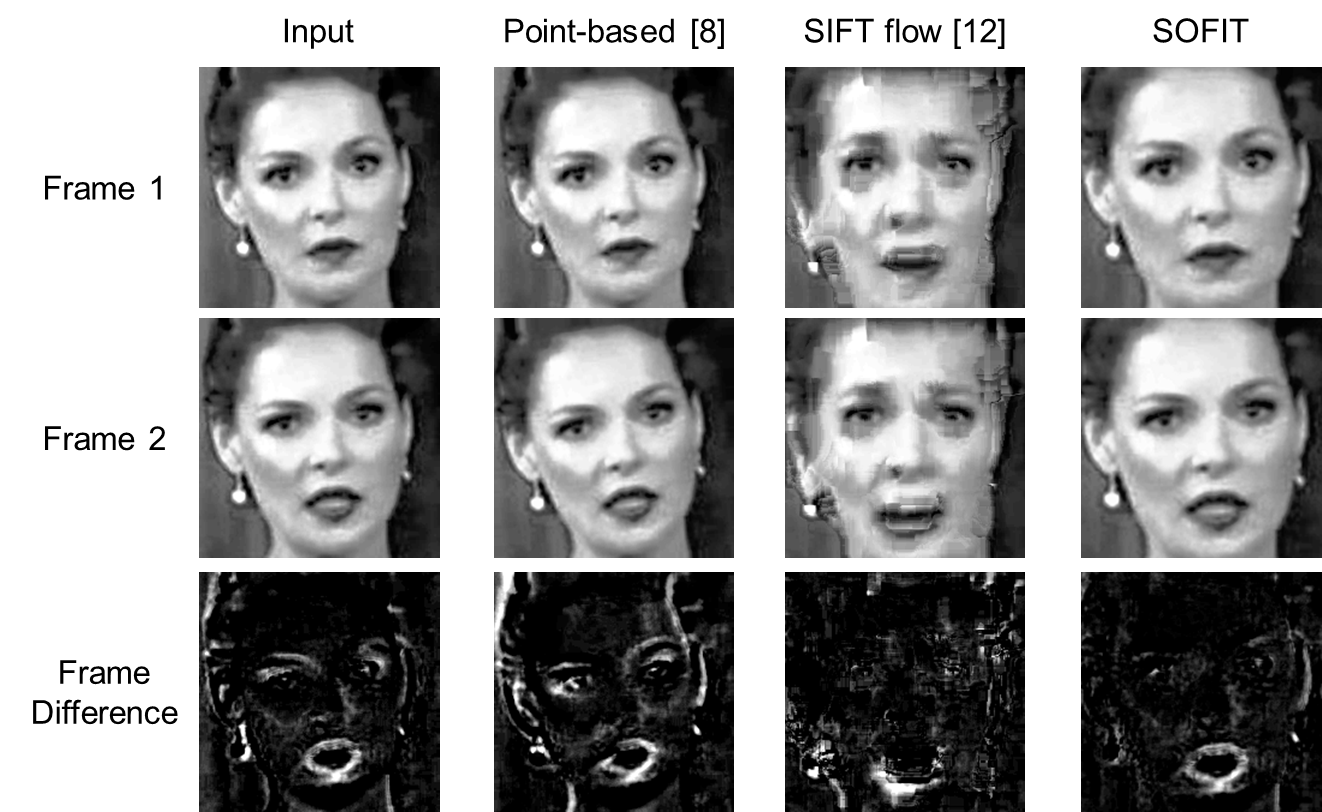
\includegraphics[width=\columnwidth]{fig/regComp.png}
	\caption{Comparison of registration results. Row 3 is the absolute difference between frame 1 and frame 2. Column 2 is the point-based affine registration method used in~\cite{Littlewort_CERT_FG2011,Tadas_ECCV14,Valstar_SMCB12,IntraFace,McDuff_TAC14}, where affine (or piece-wise affine) transformation is computed from 83 facial feature points generated by the state-of-the-art detector~\cite{Tadas_ECCV14}. Column 3 uses SIFT flow~\cite{Liu_PAMI11} to align with the Avatar Reference face model from~\cite{Yang_SMCB12}. Ideally, we would like the frame difference to show only at locations where the non-rigid motion is present (mouth area in this case). The proposed method, SOFIT, achieves the most plausible result.}
	\label{fig:regComp}
\end{figure}

\begin{enumerate}
\item Facial expression comprises non-rigid muscle motion and rigid head motion.
\item The head pose comprises both in-plane rotation and out-of-plane rotation.
\item The muscle motion is subtle in spontaneous expressions.
\item The data are streaming instead of being in a batch form.
\item The consecutive frames should comply with temporal smoothness constraint for micro-expression analysis.
\item The imaging condition varies, such as the illumination or resolution of the face region.
%\vspace{-5pt}
\end{enumerate}

In this paper, we propose a new video registration approach, termed SIFT and Optical Flow Image Transform (SOFIT), that tackles the aforementioned challenges in aligning object features through video frames in the presence of compounded surface deformation and rigid motion.

In various tasks such as recognition, super-resolution, video compression, the deformed object should be aligned with respect to a canonical form or reference model.
For instance, such a reference model is instrumental in facial expression analysis ~\cite{Yang_SMCB12}.

Facial muscle motion is similar for the same expression irrespective of the person~\cite{Ekman78}, but the facial feature location (such as eyes, nose, mouth) of different people varies. Thus, finding a canonical reference feature location for all the faces is favorable for analyzing the dynamics of facial features across population. In other words, face registration is critical to facial expression recognition. In the proposed SOFIT approach, we need to transform every frame of the streaming video data into a canonical pose by neutralizing the effects of rigid body motion on the deformable object.

To further clarify the aforementioned design objective, let us examine, via Fig.~\ref{fig:regComp}, how different video registration methods behave when being applied to registering frame 2 with respect to frame 1.  All methods in Fig.~\ref{fig:regComp} are able to account for the in-plane head rotation. However, as illustrated by the frame difference images (row 3) for the point-based affine (or piece-wise affine) transformation (column 2) and the SIFT flow transformation (column 3), there is motion on most parts of the face. This is similar to the unaligned face image (column 1) where the image is the output of Viola-Jones face detector~\cite{Viola_IJCV04}. This suggests us to impose the temporal smoothness constraint so that the frame difference is small for areas with no motion; while for areas with motion (mouth area in this case), the frame difference should capture this change, as demonstrated by the results of the proposed method (column 4).

In this paper, we model the alignment-of-compound-motion problem in three steps. \textit{First}, each frame is aligned with respect to a reference frame in a general distance measure, which is then instantiated to the SIFT flow criterion, thereafter. \textit{Second}, our model enforces a smoothness constraint on adjacent frames. It is realistic for the consecutive frames to comply with the smoothness constraint. We realize this by depending this current transformation estimation on a number of previous frames in an optical flow criterion. \textit{Third}, large transformation is penalized to prevent over-fitting. We also extend this approach to register many other types of objects and demonstrate applications in areas such as image super-resolution. More results can be found on our project website~\footnote{\url{http://www.ee.ucr.edu/~syang/sofit/index.html}}.

The rest of the paper is organized as follows. After reviewing the related work and highlighting our contribution in Section~\ref{sec:relatedWork_Contribution}, Section~\ref{sec:approach} presents our general model as well as the solution to the registration problem using the dense flow approximation to estimate the affine transformation parameters. The experimental results and discussions are provided in Section~\ref{sec:experiment}. Finally the conclusion is drawn in Section~\ref{sec:conclusion}.


%-------------------------------------------------------------------------
\section{\label{sec:relatedWork_Contribution}Related Work and Contributions}

\subsection{\label{sec:related_work}Related Work}

Video registration has been a fundamental topic in computer vision and image processing. As an object may undergo a complex motion (rigid and/or non-rigid), conventional video registration methods~\cite{Uenohara95}~\cite{Caspi_PAMI02} attempt to correct both types of motion. On the contrary, we attempt to remove the rigid motion while retaining and characterizing the non-rigid motion. Such problem occurs when a moving object has deformable surface, which may contain crucial information (\textit{e.g.} facial expression).

To analyze facial expressions, behavioral scientists have developed Facial Action Coding System (FACS)~\cite{Ekman78} as an objective standard to describe the muscle motion. According to FACS, human (coders) can decompose every possible facial behavior into Action Units (AU), which roughly correspond to the muscles that produce them. Automatic AU recognition~\cite{Zhao_PAMI07}\cite{Valstar_SMCB12}, has been quite successful for well-aligned, posed data, such as MMI~\cite{Pantic_ICME05} and CK+~\cite{Kanade_FG00}. Unfortunately, AU recognition in an uncontrolled real-world environment remains a difficult problem, as shown in the Facial Expression Recognition and Analysis Challenge (FERA2011~\cite{Valstar_FERA11} and FERA2015~\cite{FERA15}), due to the difficulties mentioned in Section~\ref{sec:intro}. Existing face registration approaches attempt to solve different aspects of the aforementioned challenges. In the face recognition and image retrieval communities, researchers attempt to discard the non-rigid motion from facial data through registration using an ensemble of images~\cite{LearnedMiller_PAMI06}\cite{Huang_ICCV07}\cite{Peng_PAMI12}. These approaches are not suitable in the facial expression recognition domain, where the following three criteria should be met:
\begin{enumerate}
\item Non-rigid facial muscle motion, which carries essential information for expression inference, should be retained. 
\item Facial features should be aligned under various muscle motions and pose variations. 
\item Subtle facial muscle motion should be captured for spontaneous facial expression analysis.
\end{enumerate}

To align faces with expressions, the state-of-the-art systems~\cite{Valstar_SMCB12,Littlewort_CERT_FG2011,Tadas_FERA15} track a set of anchor points on the face and estimate the affine transformation based on which the entire face is warped. Although the most recent facial point detection techniques~\cite{Martinez_PAMI13,Xiong13,Zhu_CVPR12,Tadas_ECCV14} are able to achieve accurate detection results, there are two significant issues that need to be addressed. \textit{First of all}, the affine estimation is sensitive to small perturbation of point detection results. Typically in point-based method, a number of facial fiducial points (\textit{e.g.}, 20 points in~\cite{Valstar_SMCB12} and~\cite{Martinez_PAMI13}) are detected. Each point carries much more weights in the estimation of the affine transformation matrix compared with methods that use corresponding information from the entire image, as demonstrated by Fig.~\ref{fig:regComp}. \textit{Besides}, affine transform parameter estimation by a small set of points can be susceptible to detection errors. In a realistic case where the resolution of the face is not high enough, the accuracy of feature point detection will also degrade. Yang and Bhanu~\cite{Yang_SMCB12} adopted SIFT flow technique~\cite{Liu_PAMI11} to align every frame to a reference face. As shown in Fig.~\ref{fig:regComp}, column 3, the outcome of the SIFT flow transform displays a large amount of discontinuities and artifacts. Although they attempt to solve this issue by generating image-based face representations (\textit{i.e.}, Emotion Avatar Image) and a reference model (\textit{i.e.}, Avatar Reference), carrying out the double layer loopy-belief propagation in SIFT flow for every frame is computationally expensive and not suitable for real-time systems.

\subsection{\label{sec:contribution}Contributions of This Paper}

The contributions of this work are summarized as follows:

\begin{enumerate}
\item Unlike methods in the registration literature that attempt to correct the motion, we attempt to solve a more challenging problem: aligning objects under compound motion, in the hope of compensating the rigid motion while retaining the non-rigid motion.
\item We propose a novel real-time streaming registration framework, SOFIT, that aligns the objects under compound motion. SOFIT is a holistic approach and no detection of local features (eyes, nose, mouth) is needed. Therefore, it is robust against noise, detection error, and low image resolution. The proposed method results in temporally smooth and aligned image sequences.
\item We quantitatively demonstrate the versatility of our registration method in the fields of spontaneous AU recognition and image super-resolution. We also show results for generic object alignment under various challenges.
\end{enumerate}



%-------------------------------------------------------------------------
\section{\label{sec:approach}Flow-based Real-time Object Registration}

The objective of this work is to align objects in video in an uncontrolled environment. Taking face images as specific examples, the original inputs to our system can be faces detected by the Viola-Jones detector~\cite{Viola_IJCV04} for the analysis and illustrations in expression analysis domain. We first formulate the generalized model in a Bayesian framework. A flow-based approximation results in an efficient closed-form solution. We also point out a dynamic programming implementation that will further optimize the registration algorithm.

\subsection{\label{sec:model}The Generalized Model}

Let $p$ be the grid coordinate of $I_i$, the $i$-th frame in grayscale. For simplicity, we write the intensity of an image, $I_i$, as a shorthand for $I_i(p)$. Given a sequence of $N$ unregistered frames of an object, our goal is to align individual frames with respect to a canonical representation of this object, denoted by $I_c$. Let $w_i$ be the flow field to register frame $i$, then the $i$-th registered frame can be written as $I_i(p+w_i)$. To align the entire sequence, the objective is to recover $w_1,\ldots,w_N$ for each of the $N$ images in the sequence.  We model the distance measurement of $I_i(p+w_i)$ and $I_c$ as a random variable $Q_i$ corrupted by a Gaussian noise $m_Q$. Thus,

\begin{align}
\label{model:measurement}
Q_i=Dist(I_i(p+w_i),I_c)+m_Q,
\end{align}

\noindent where $Dist(\cdot,\cdot)$ is a generic distance function. In this paper, we attempt to align every frame with respect to the canonical representation such that they share similar structure. However, in general, it is applicable to many other distance measures. $m_Q$ is i.i.d. (\textit{i.e.}, independent and identically distributed) normally distributed zero-mean measurement noise. We model the measurement of the transformation, $w_i$, as a random variable $Y_i$. The difference between $Y_i$ and $w_i$ is modeled by an i.i.d zero-mean Gaussian distribution:

\begin{align}
\label{model:penalty}
Y_i=w_i+m_Y,
\end{align}

\noindent where $w_i$ is the underline true variable we intend to solve. This model penalizes excessive transformation due to over-fitting. The joint probability of all variables can be written as

\begin{equation}
\begin{aligned}
L&=P(w_{1:N},Y_{1:N},Q_{1:N},I_c) \\
 &=P(Q_{1:N},Y_{1:N}|w_{1:N},I_c,)P(w_{1:N}|I_c)P(I_c),
\end{aligned}
\end{equation}

\noindent where $w_{1:N}$ is short for $w_1,\ldots,w_N$. Dropping the constant term and using the independence of our model definition in Eq.~\eqref{model:measurement} and~\eqref{model:penalty}, we obtain

\begin{equation}
\begin{aligned}
L\propto & P(Q_{1:N}|w_{1:N},I_c) P(Y_{1:N}|w_{1:N}) P(w_{1:N}) \\
				=& \prod_{i=1}^N{P(Q_i|w_i,I_c)} \prod_{i=1}^N{P(Y_i|w_i)} \prod_{i=1}^N {P(w_i|w_{1:i-1})},
\label{model:joint}
\end{aligned}
\end{equation}

\noindent where $\prod_{i=1}^N {P(w_i|w_{1:i-1})}$ can be viewed as the smoothness constraint. With the weakly coupled Markov assumption, we only take into account $H=min(i,h)$ number of frames prior to frame $i$. The assumption is that the aligned frame $I_i$ should have similar appearance with its previous $h$ neighbors (if $h<i$). With the models in Eq.~\eqref{model:measurement} and~\eqref{model:penalty} as the prior terms in Eq.~\eqref{model:joint}, the joint probability can be written as 

\begin{align}
L\propto & \prod_{i=1}^N{P(Q_i|w_i,I_c)} \prod_{i=1}^N {P(w_i|w_{i-H:i-1})} \prod_{i=1}^N{P(Y_i|w_i)} \\
\label{data_exp}
				=& \prod_{i=1}^N \frac{1}{\sigma \sqrt{2\pi}} \exp\{-\frac{1}{2\sigma}Dist(I(p+w_i),I_c)\}  \\
\label{smooth_exp}
				\times &\prod_{i=1}^N \frac{1}{\epsilon \sqrt{2\pi}} \exp\{-\frac{1}{2\epsilon H}\sum_{j=1}^{H}\parallel{I_i(p+w_i)-I_{i-j}(p+w_{i-j})}\parallel_F^2\} \\
\label{penalty_exp}
				\times &\prod_{i=1}^N \frac{1}{\tau \sqrt{2\pi}} \exp\{-\frac{1}{2\tau}\parallel{w_i}\parallel_F^2\},
\end{align}


\noindent where $\parallel \cdot \parallel_F$ is the Frobenius norm; the smoothness constraint $P(w_i|w_{i-H:i-1})$ obeys zeros-mean Gaussian distribution; $\sigma$, $\epsilon$, $\tau$ control the variance for the corresponding Gaussian distribution. Maximizing the likelihood, $L$, is equivalent to minimizing its negative log likelihood, $E$, where

\begin{align}
\label{data}
E = &\sum_{i=1}^{N}Dist(I_i(p+w_i),I_c) \\
\label{smooth}
	+ &\frac{\alpha}{2H}\sum_{i=1}^{N}\sum_{j=1}^{H}\parallel{I_i(p+w_i)-I_{i-j}(p+w_{i-j})}\parallel_F^2 \\
\label{penalty}
	+ &\frac{\beta}{2}\sum_{i=1}^{N}\parallel{w_i}\parallel_F^2,
\end{align}


\noindent where the constant terms are dropped. $\alpha=\sigma^2 / \epsilon^2$ and $\beta=\sigma^2 / \tau^2$ can be considered as two scaling parameters on the smoothness term and penalty term, respectively. 

\subsection{The Flow-based Instantiation}

The $Dist$ function in Eq.~\eqref{data} measures the similarity between two images. One can define its form according to different applications. Since our objective is structural matching, we opt to use SIFT flow \cite{Liu_PAMI11} for similarity matching under large, non-rigid transformation. SIFT flow \cite{Liu_PAMI11} was originally designed to align an image to its plausible nearest neighbor which can have large variations. The SIFT flow algorithm matches dense SIFT features~\cite{SIFT} between two images, resulting in a structural coherent image pairs. Although SIFT flow by itself generates block artifacts, it includes a structural matching constraint that allows non-rigid motion correspondence. Thus, the data matching term in Eq.~\eqref{data} can be instantiated in the coordinate space as

\begin{align}
\label{data_sift}
&\sum_{i=1}^{N}Dist(I_i(p+w_i),I_c)=\sum_{i=1}^{N}\parallel{w_i-f_s^i}\parallel_F^2,
\end{align}

\noindent where $f_s^i$ (shorthanded for $f_s(I_i,I_c)$) is the pixel-wise SIFT flow field given by matching $I_i$ to canonical reference frame $I_c$. The reference frame of face images is chosen to be the Level-1 Avatar Reference (AR) image~\cite{Yang_SMCB12} generated from the FERA-GEMEP dataset~\cite{Valstar_FERA11}. AR is essentially a face model that reflects the expression and identity of the entire population in the dataset. It is computed offline by an iterative algorithm that estimates the reference model and the individual expression model simultaneously. It has been demonstrated to perform well across datasets~\cite{Yang_SMCB12}. For different classes of objects, the canonical image representation is generated in the same way.

Regarding the smoothness constraint in Eq.~\eqref{smooth}, we consider the optical flow between frames. Optical flow computes the motion between two frames by matching the corresponding intensity values. In the context of video processing, it is reasonable to assume that the frame rate is high enough for computing accurate optical flow between consecutive frames. With the pixel-level correspondence, we can approximate the current frame by its previous frame, \textit{i.e.}, $I_i\simeq I_{i-j}(p+f_o^{i-j,i})$, where $f_o^{i-j,i}$ is the optical flow field from frame $i-j$ to frame $i$. Thus, applying the corresponding registration transformation on both sides yields

\begin{equation}
\begin{aligned}
\label{eq:smooth_inter}
I_i(p+w_i)& \simeq I_{i-j}(p+f_o^{i-j,i}+w_{i-j}) \\
					& \simeq I_{i-j}(p+f_o^{i-j,i}+f_s^{i-j}).
\end{aligned}
\end{equation}

The approximation in the second line of Eq.~\eqref{eq:smooth_inter} holds true according to the structural constraint in Eq.~\eqref{data_sift}. Once again, due to the illumination invariant assumption under high frame rate for optical flow, Eq.~\eqref{eq:smooth_inter} is equivalent to

\begin{equation}
\begin{aligned}
w_i \simeq f_o^{i-j,i}+f_s^{i-j}.
\end{aligned}
\end{equation}

Therefore, the smoothness constraint in Eq.~\eqref{smooth} can be rewritten as

\begin{equation}
\begin{aligned}
\label{smooth_opt}
&\frac{\alpha}{2H}\sum_{i=2}^{N}\sum_{j=1}^{H}\parallel{I_i(p+w_i)-I_{i-j}(p+w_{i-j})}\parallel_F^2 \\
&\simeq\frac{\alpha}{2H}\sum_{i=2}^{N}\sum_{j=1}^{H}\parallel{w_i-(f_o^{i-j,i}+f_s^{i-j})}\parallel_F^2.
\end{aligned}
\end{equation}


Now, the cost function is written as the sum of three $\ell_2$ norm terms in Eq.~\eqref{data_sift},~\eqref{smooth_opt}, and~\eqref{penalty}. Since the speed of the algorithm is a main concern for real-time applications in practice, we adopt $\ell_2$ norm in our formulation, such that a closed-form solution for this optimization problem can be derived. We further assume that the transformation function is affine. The computation of the $X,Y$-component can be decomposed, which enables speedup using parallel computation. Thus, the cost function is instantiated as

\begin{align}
	\label{data_affine}
E		=&\frac{1}{2}\sum_{i=1}^{N}\parallel{T_ip-p-f_s^i}\parallel_F^2
\\\label{smooth_affine}
				+&\frac{\alpha}{2H}\sum_{i=2}^{N}\sum_{j=1}^{H}\parallel{T_ip-p+(f_o^{i-j,i}+f_s^{i-j})}\parallel_F^2
\\\label{penalty_affine}
				+&\frac{\beta}{2}\sum_{i=1}^{N}\parallel{T_ip-p}\parallel_F^2,
\end{align} 

\noindent where the flow $w_i$ is written as $T_ip-p$; $T_i$ is a $3\times3$ affine matrix. With minor
 abuse of notion, $p$ is now a horizontal stacked coordinate location template of size $3\times m$, where $m=r\times c$, assuming that $r$ and $c$ are the image height and width, respectively. Each column of $p$ is a coordinate point $(x,y,1)$ in homogeneous coordinates. Taking the derivative of $E$ w.r.t. $T_i$ and setting it to zero result in 

\begin{equation}
\begin{aligned}
\label{eq:result}
T_i=&(1+\alpha+\beta)^{-1}\times \\
		&(f_s^i+\frac{\alpha}{H}\sum_{j=1}^H(f_s^{i-j}+f_o^{i-j,i})+(1+\alpha+\beta)p)p^T(pp^T)^{-1}.
\end{aligned}
\end{equation}

It is observed from Eq.~\eqref{eq:result} that for every input frame $I_i$, we have to compute its SIFT flow with respect to the canonical reference frame. Computing SIFT flow for every frame is time-consuming. However, given accurate optical flow estimation between frames (which is a practical assumption for video at high frame rate), we can approximate the SIFT flow computation of the $i$-th frame by the sum of the SIFT flow of the $(i-1)$-th frame and the optical flow from the $(i-1)$-th to the $i$-th frame, \textit{i.e.}

\begin{align}
\label{eq:approx}
f_s^i=f_s^{i-1}+f_o^{i-1,i},
\end{align}

Therefore, the final closed-form solution can be written as

\begin{align}
\label{eq:final}
T_i=&(1+\alpha+\beta)^{-1}\times \nonumber \\
		&(f_s^{i-1}+f_o^{i-1,i}+\frac{\alpha}{H}\sum_{j=1}^H(f_s^{i-j}+f_o^{i-j,i})) + I_3, \nonumber \\
\end{align}

\noindent where $I_3$ is a $3\times 3$ identity matrix. Eq.~\eqref{eq:final} can be rewritten as

\begin{align}
\label{eq:dp}
T_i=T_{i-1}+(1+\alpha+\beta)^{-1}(f_o^{i-1,i}+\frac{\alpha}{H}g) + I_3,
\end{align}

\noindent where $g=f_s^{i-1}-f_s^{i-H-1}+\sum_{j=1}^H(f_o^{i-j,i}-f_o^{i-j-1,i-1})$. It can be seen that Eq.~\eqref{eq:dp} is written in a typical dynamic programming (DP) formulation, where we can cache the previously computed SIFT and optical flows. For the current frame $i$, we only carried out several optical flow computations, \textit{i.e.}, $f_o^{i-H,i},\ldots,f_o^{i-1,i}$. When $H$ is small, \textit{e.g.}, $3$-$5$, the optical flow is accurate and the total amount of optical flow computation is small. The DP implementation dramatically reduces the computational cost and enables real-time execution of our algorithm. Besides, individual optical flow can be computed in parallel to further speed up the algorithm. What's more, we use Iteratively Reweighted Least Squares (IRLS)~\cite{Huber81} to robustly estimate the affine transformation matrix. 

\begin{figure}[htbp]
	\centering
		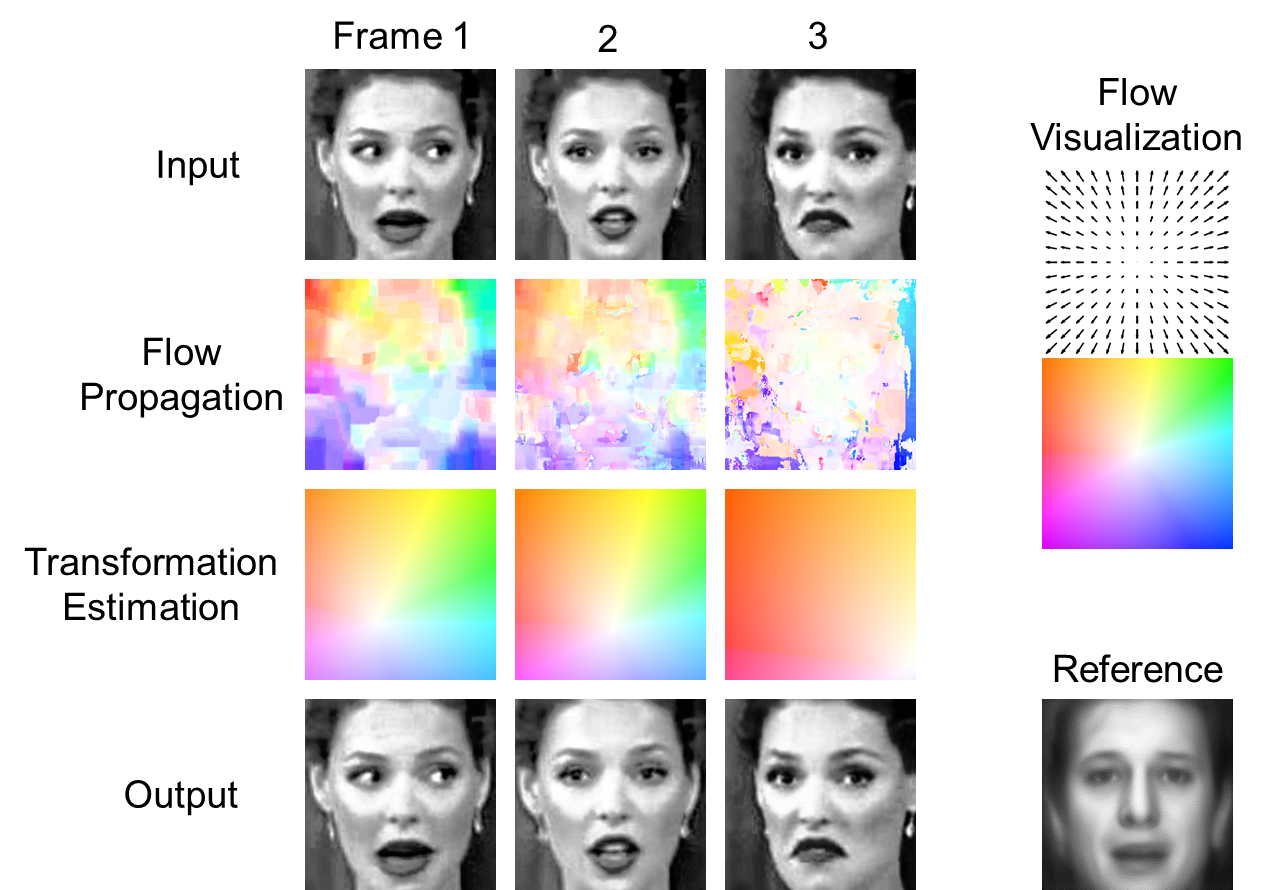
\includegraphics[width=\columnwidth]{fig/theory_example.png}
	\caption{SOFIT registration example. The input sequence is registered with respect to the reference frame shown on the bottom right. The flow visualization is coded as in~\cite{Baker_ICCV07}. Better viewed in color.}
	\label{fig_theory_example}
\end{figure}

A registration example for face is visualized in Fig. \ref{fig_theory_example}. The flow propagation, computed by Eq.~\eqref{eq:final}, is visualized in the second row for consecutive frames. The affine transformation is then robustly estimated for each frame. The output sequence is registered with respect to the reference frame and exemplar frames comply with smoothness constraint. 


\subsection{\label{sec:details}Error Propagation and Loop-closure Rectification}

In our model, we make a compromise between model optimality and computation efficiency. Therefore, the average registration error accumulates over time. The registration error is defined as the deviation from the canonical reference frame. Since we care about structural similarity, we compute the mean length of the SIFT flow from the current frame to the reference frame. For error analysis, we need videos with length of more than one minute ($1800$ frames in our case with $30$ fps) to observe the noticeable cumulative error. Therefore, we register a long video sequence\footnote{source: \url{https://www.youtube.com/watch?v=_aKNYRwb4-4}} and plot the error in Fig.~\ref{fig_error_prop}. Although this error measurement consists of both global rigid head motion and local non-rigid muscle motion, we are still able to observe the error accumulation effect.

\begin{figure}[htbp]
	\centering
		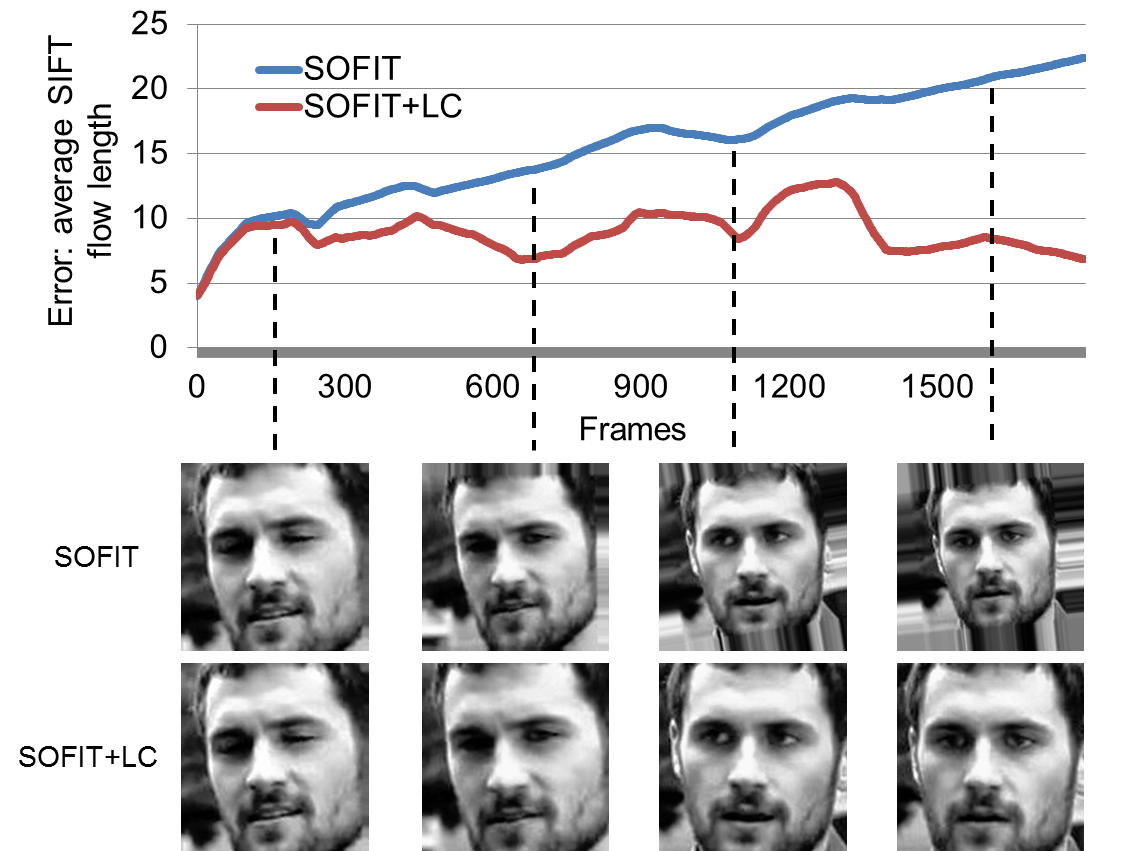
\includegraphics[width=.9\columnwidth]{fig/error_prop.png}
	\caption{The error accumulation over time. The error is defined as the SIFT flow of the current frame to the canonical reference frame. We use loop-closure (LC) to update the global flow estimation and rectify the error. The LC is carried out every $300$ frames in this experiment.}
	\label{fig_error_prop}
\end{figure}

To solve this issue, we intend to update the global estimation at a certain rate without affecting the propagation computation. Inspired by the Loop-Closure (LC) strategy in robotics \cite{close_loop_icra_05}, we update $f_s$ in Eq.~\eqref{eq:final} by recomputing the SIFT flow for every $300$ frames. This update frequency is chosen because cumulative error is negligible within $300$ frames based on empirical observations, and this also provides enough time for $f_s$ to be updated in parallel and will not affect the overall flow propagation. As seen in Fig. \ref{fig_error_prop}, the error is rectified by the global flow estimation update. 


\subsection{\label{sec:time}Computational Cost Analysis}
We obtain considerable speedup using dynamic programming based implementation. In essence, the SIFT flow only needs to be computed for the initialization. The steps to be carried out for every subsequent frame are the following:
\begin{enumerate}
\item Compute the dense optical flow with respect to the previous $H$ frame in parallel.
\item Estimate affine transformation matrix using Eq.~\eqref{eq:final} based on the updated coordinate value.
\end{enumerate}

We adopt the optical flow implementation in OpenCV~\cite{opencv}. The aforementioned steps can be finished in approximately $47$ms on average for a $100\times100$ image on a quad-core Intel i7 4GHz machine with 32GB memory. In other words, the execution speed reaches 21 fps under this setting. Since the bottleneck of our method is optical flow computation, one can further speedup the algorithm by GPU implementation. The initialization takes on average about $1.2$ second using the aforementioned settings. The computation of SIFT flow and optical flow are also in parallel. The LC re-initialization is also in parallel with the the optical flow computation, and it will not affect the speed of the registration procedure. 


%---------------------------------------------------------------
\section{\label{sec:experiment}Experimental Results}

In this section, we show results on two applications of the proposed method, including facial AU recognition and image super-resolution. For AU recognition, we follow the challenge guideline of FERA2011 and FERA2015 for a thorough analysis and comparison. In addition, we have also included qualitative results on different types of objects to demonstrate the generalizability of our approach.

\subsection{Facial Action Unit Recognition}

The goal of AU recognition is to detect a set of frequently occurring AUs on a per-frame basis. The main concerns here are two-fold:
\begin{enumerate}
\item Is registration really an important issue in real-world AU recognition in uncontrolled environment?
\item If yes, can we improve the recognition performance just by adopting a better registration algorithm, \textit{e.g.}, SOFIT?
\end{enumerate}

\noindent \textbf{Datasets: FERA-GEMEP}

We first demonstrate SOFIT face registration technique by facial AU recognition on FERA Challenge 2011 dataset~\cite{FERA11}. We use the same protocol as the FERA2011~\cite{Valstar_FERA11} AU sub-challenge. The data we use for training is the GEMEP-FERA training dataset, which includes 87 sequences and around 5400 frames. The pose and gesture of the subjects in this dataset are uncontrolled, and therefore, this dataset is more realistic and complex compared to the legendary MMI~\cite{Pantic_ICME05} and CK+~\cite{Kanade_FG00} datasets.

To address the aforementioned issues, we use the exact same features as in the baseline approach for a fair comparison. The only variable in our experiment design is using different registration methods. The \textit{baseline} registration method detects both eye locations on the faces, and then unifies their scales, and in-plane rotations. This registration belongs to in-plane image transformation category as summarized in~\cite{Yang_SMCB12}. A typical point-based registration method tracks facial landmarks and estimates the affine (or piece-wise affine) transformation based on a set of rigid landmarks such as eye corners or nose~\cite{Littlewort_CERT_FG2011,IntraFace,McDuff_TAC14}. We term this family of methods as point-based affine (\textit{PA}), and we use piece-wise affine in our experiment. Another registration technique in comparison is the Emotion Avatar Image (\textit{EAI})~\cite{Yang_SMCB12}, which achieves the best performance in FERA Challenge 2011.


\begin{table*}[htbp]
\caption{Person-independent AUC-score result on FERA-GEMEP AU training set}
\begin{center}
\label{table:fera}
\begin{tabular}{ccccccccccccccc}
\toprule
& & AU1 & AU2 & AU4 & AU6 & AU7 & AU10 & AU12 & AU15 & AU17 & AU18 & AU25 & AU26 & Avg.	\\ 
\midrule
\multirow{2}{*}{BaseLine~\cite{Valstar_FERA11}}	& LBP 		&0.69	&0.69	&0.58	&0.68	&0.61	&0.68	&0.68	&0.52	&0.61	&0.57	&0.53	&0.52	&0.61 \\
																								& LBP-TOP &0.70	&0.69	&0.61	&0.74	&0.66	&0.64	&0.77	&0.51	&0.61	&0.60	&0.55	&0.53	&0.63 \\
																								\midrule
\multirow{2}{*}{PA~\cite{Tadas_ECCV14}}					& LBP 		&0.69	&0.69	&0.63	&0.69	&0.62	&0.65	&0.72	&0.55	&0.65	&0.66	&0.56	&0.56	&0.64 \\
																								& LBP-TOP &0.67	&0.69	&0.73	&0.73	&\textbf{0.69}\cellcolor[gray]{0.9}	&0.64	&0.70	&0.66	&0.59	&\textbf{0.77}\cellcolor[gray]{0.9}	&0.53	&0.51	&0.66 \\
																								\midrule
\multirow{2}{*}{EAI~\cite{Yang_SMCB12}}					& LBP 		&0.68	&0.68	&0.68	&0.69	&0.62	&0.61	&0.75	&0.54	&0.66	&0.72	&0.55	&0.56	&0.65 \\
																								& LBP-TOP &0.71	&\textbf{0.71}\cellcolor[gray]{0.9}	&0.61	&0.66	&0.63	&0.66	&0.78	&0.67	&0.67	&0.69	&0.51	&0.52	&0.65 \\
																								\midrule				
\multirow{2}{*}{SOFIT}													& LBP 		&\textbf{0.76}\cellcolor[gray]{0.9}	&0.70	&0.62	&0.78	&0.67	&\textbf{0.70}\cellcolor[gray]{0.9}	&0.74	&\textbf{0.68}\cellcolor[gray]{0.9}	&\textbf{0.69}\cellcolor[gray]{0.9}	&0.74	&\textbf{0.57}\cellcolor[gray]{0.9}	&0.58	&0.69 \\
																								& LBP-TOP &0.73	&0.70	&\textbf{0.75}\cellcolor[gray]{0.9}	&\textbf{0.80}\cellcolor[gray]{0.9}	&0.64	&0.67	&\textbf{0.82}\cellcolor[gray]{0.9}	&\textbf{0.68}\cellcolor[gray]{0.9}	&0.67	&0.76 &\textbf{0.57}\cellcolor[gray]{0.9}	&\textbf{0.63}\cellcolor[gray]{0.9}	&\textbf{0.70}\cellcolor[gray]{0.9} \\
\bottomrule
\end{tabular}
\end{center}
\end{table*}


The feature extraction and classification are conducted in the same way as the baseline approach. After extracting the faces from Viola-Jones detector~\cite{Viola_IJCV04}, we register all faces using the aforementioned methods. All registered face images are all of size $100\times100$. Subsequently, we divide the image into $10\times10$ blocks, where static features, Local Binary Pattern (LBP)~\cite{Ojala_PAMI02}, and dynamic feature, LBP in three orthogonal planes~\cite{Zhao_PAMI07} (LBP-TOP), for each block are computed and concatenated separately. We then train $12$ linear SVM binary classifiers based on the implementation of~\cite{SVMlib}, each of which is trained independently regardless of the co-occurrence of AUs.

Concretely, the feature dimensions are the following:
\begin{enumerate}
\item LBP: the uniform LBP operator generates 59 basic patterns for a local patch. Given our region segmentation settings, the total feature dimension is $59\times 10\times 10=5900$. 
\item TOP-LBP: since the feature dimension enlarges by a multiple of $3$ compared with LBP, the total feature dimension is $3\times 5900=17700$.
\end{enumerate} 



For registration methods with reference frame, \textit{i.e.}, EAI~\cite{Yang_SMCB12}, and SOFIT, we use the Level-1 Avatar Reference~\cite{Yang_SMCB12} generated from the FERA Challenge training data \cite{FERA11}. To generate an EAI representation, we need to determine a temporal length parameter. In~\cite{Yang_SMCB12}, this parameter is chosen as the length of a single video (around $2$ seconds) for facial expression recognition on a per-video basis. To generalize this registration technique in AU recognition on a per-frame basis, we empirically determine the best value for the temporal length parameter. We carry out a leave-one-subject-out cross validation on the FERA-GEMEP AU training data, and find $0.56$ second is a reasonable temporal length to achieve the best F1 score over all AUs. This means that for each frame in a video, approximately $14$ consecutive frames are used to compute EAI representation. For the boundary frames, \textit{i.e.} the starting and the ending $7$ frames, we simply assign their values to be the $8$th frame from the beginning and from the end, respectively. The aforementioned features are extracted from the EAI representations thereafter.

For PA method, 83 points are tracked using~\cite{Tadas_ECCV14}. Each image is then registered by piece-wise affine warping estimated from 41 rigid points, including nose, eye corner, \textit{etc}. We only include the texture in the face region and blacken the periphery of the entire region. Since the non-face region will not interfere the classification model training, for simplicity, we include all regions for feature extraction.  

\begin{figure*}[t]
	\centering
		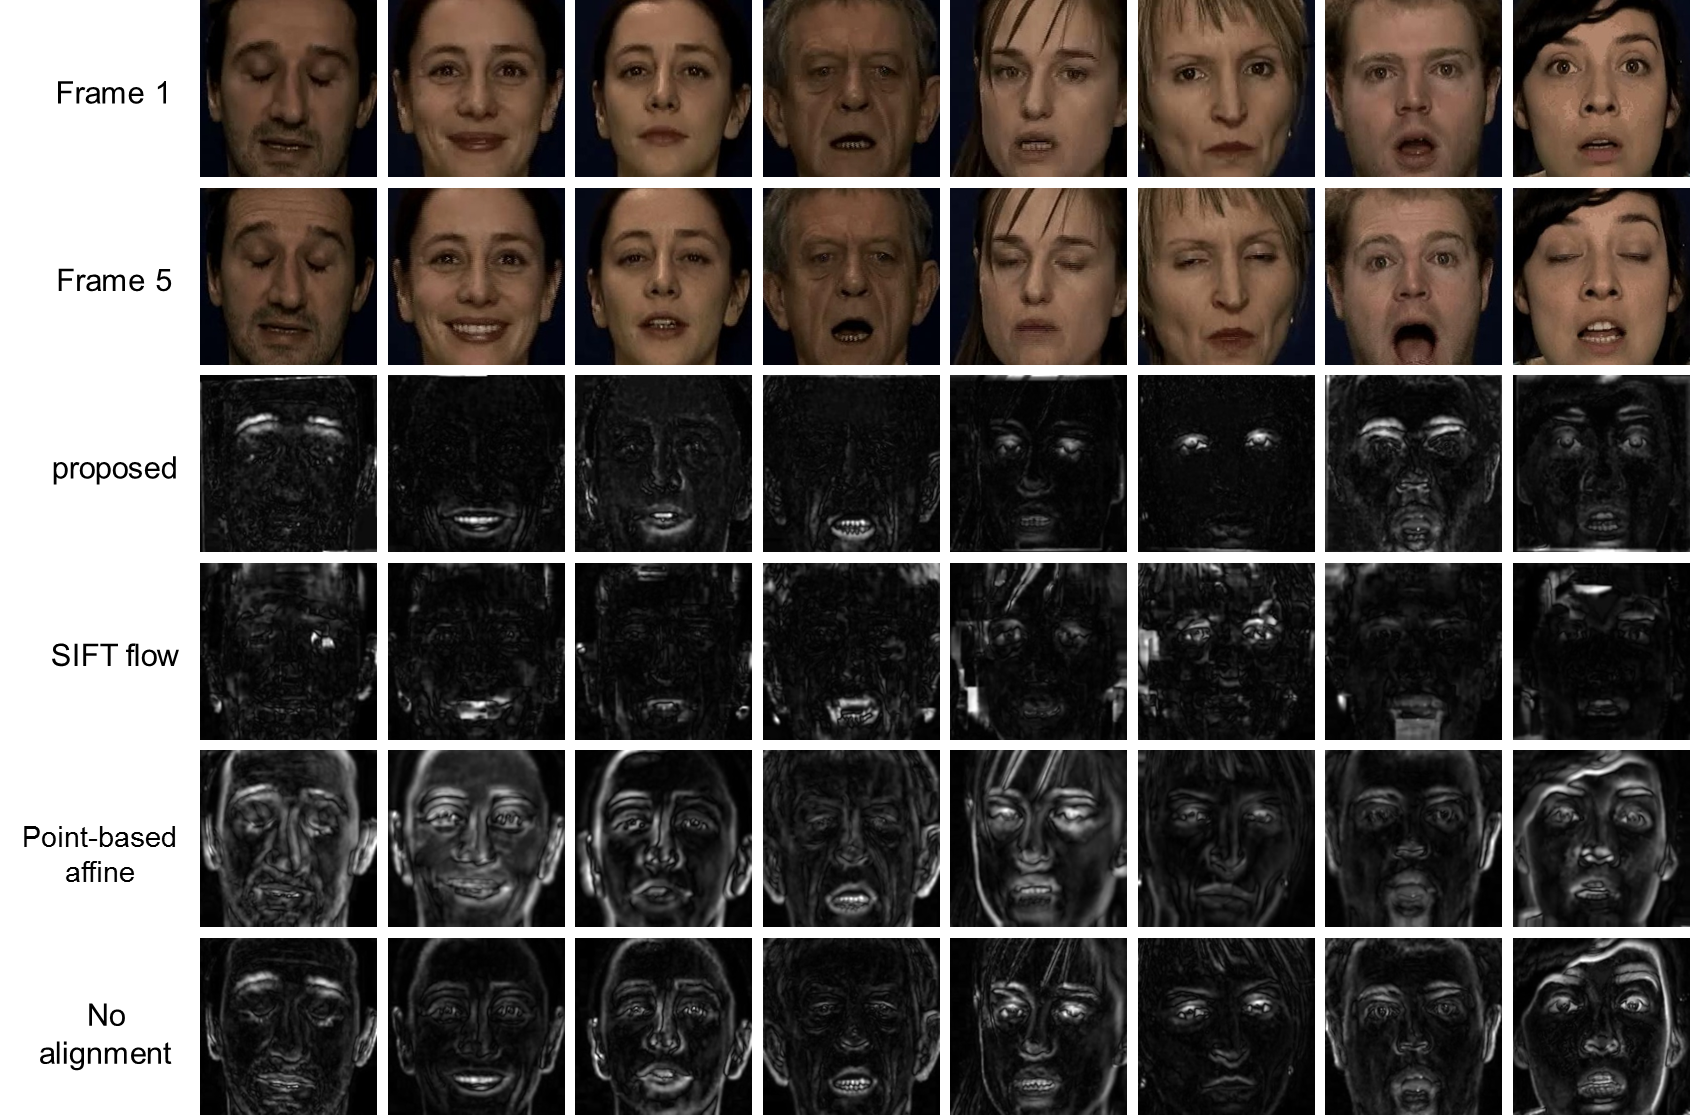
\includegraphics[width=0.8\textwidth]{fig/fera_diff.png}
	\caption{Qualitative face registration results comparison. Row 1 and 2 are the first and fifth frame of a sequence. Row 3 to 5 are the cumulative absolute frame difference of 5 unaligned frames using method SOFIT, EAI~\cite{Yang_SMCB12}, PA where points are detected using~\cite{Tadas_ECCV14}, respectively. The proposed alignment technique captures the correct non-rigid motion of face, for example, eyebrows raise for first column and mouth open for second column.}
	\label{fig:fera_diff}
\end{figure*}


Since the ground-truth label is only available for the FERA-AU training set, we carry out a person-independent cross validation experiment, such that no test subject is used for training, and the average performance is reported. Due to the finite scale of the training exemplars, person-independent test is essential to demonstrate the generalization ability of an approach to unseen subjects. Table~\ref{table:fera} shows the performance obtained using both LBP and LBP-TOP feature extractors, respectively. The area under curve (AUC) score of the receiver operating characteristic (ROC) curve is reported. As seen from Table~\ref{table:fera}, on average, SOFIT outperforms the other methods by a significant margin using both LBP and LBP-TOP features. SOFIT achieves the best performance in 9 out of 12 AU classification tasks. In general, LBP-TOP outperforms LBP likely due to the dynamic information extracted. EAI is on par with PA in terms of the average AUC score. EAI performs well in categorical emotion recognition~\cite{Yang_SMCB12}; in a per-frame based setting, however, EAI lacks the ability to maintain the subtle muscle motion. Moreover, dynamic feature is not advantageous in the EAI case. A plausible explanation is that the inherent dynamics are buried in the block artifacts caused by SIFT flow. We should point out that the video sequences in FERA-GEMEP is relatively short, \textit{i.e.} around 2 seconds. Thus, the propagation error is negligible and thus we exclude the loop closure rectification procedure in this experiment. 

\noindent \textbf{Datasets: BP4D}


\begin{table*}[htbp]
\caption{Person-independent F1-score on BP4D development set (2D data only)}
\begin{center}
\label{table:bp}
\begin{tabular}{cccccccccccccc}
\toprule
& AU1 & AU2 & AU4 & AU6 & AU7 & AU10 & AU12 & AU14 & AU15 & AU17 & AU23 & Avg.	\\ 
\midrule
BaseLine~\cite{FERA15}	&0.35	&0.26	&0.40	&0.77	&0.74	&0.78	&0.81	&0.60	&0.25	&0.52	&0.26	&0.52 \\
PA~\cite{Tadas_ECCV14}					&0.36	&0.26	&0.42	&0.70	&0.74	&0.81	&0.84	&0.60	&\textbf{0.36}\cellcolor[gray]{0.9}	&0.58	&0.35	&0.55 \\
EAI~\cite{Yang_SMCB12}					&0.38	&0.27	&\textbf{0.47}\cellcolor[gray]{0.9}	&0.78	&0.78	&0.82	&0.82	&0.60	&0.35	&0.60	&0.31	&0.56 \\
SOFIT														&\textbf{0.41}\cellcolor[gray]{0.9}	&\textbf{0.32}\cellcolor[gray]{0.9}	&0.45	&\textbf{0.80}\cellcolor[gray]{0.9}	&\textbf{0.80}\cellcolor[gray]{0.9}	&\textbf{0.86}\cellcolor[gray]{0.9}	&\textbf{0.89}\cellcolor[gray]{0.9}	&\textbf{0.62}\cellcolor[gray]{0.9}	&0.35	&\textbf{0.61}\cellcolor[gray]{0.9}	&\textbf{0.36}\cellcolor[gray]{0.9}	&\textbf{0.59}\cellcolor[gray]{0.9} \\
\bottomrule
\end{tabular}
\end{center}
\end{table*}


We also carry out experiments on the BP4D~\cite{BP4D} dataset, which is also used by the FERA2015 challenge~\cite{FERA15}. It is a spontaneous facial expression dataset collected in an lab setting with uncontrolled pose and gesture. It contains 41 subjects participating in 8 tasks, which are designed to solicit expressions that are not deliberately posed. The subjects are aging from 18 to 29 covering various ethnicity groups. The original dataset includes both 2D and 3D videos, and we only use the 2D videos in our experiment. The dataset is partitioned into \textit{Training} and \textit{Development} sets with the ground truth label available. Similar to the FERA-GEMEP dataset, the ground truth label of each frame is obtained according to the FACS. Each subject has 8 sessions, and there are 168 sessions in the training and 160 sessions in the development partition, each of which has over $70k$ images.

In FERA2015, the performance is measured by the $F1$ score, calculated as:

\begin{align}
F_1 = \frac{2PR}{P+R}
\end{align}

\noindent where $P$ and $R$ represents the precision and recall, respectively.

The challenge baseline system uses Viola-Jones face detector and directly extract the appearance feature, Local Binary Gabor Patterns (LGBP)~\cite{LGBP}. LGBP is essentially the LBP features extract from the Gabor filter magnitude response of the original image, resulting a $16,992$ feature dimension for each frame. The feature dimension is then reduced by Principle Component Analysis (PCA) while keep 98\% of the energy. 

We then carry out a person-independent experiment on the training set, similar to the ones in~\cite{BP4D,FERA15}, where we follow a 10-fold cross-validation procedure and use 19 subjects for training and 2 for testing. The one-vs-all linear SVM is used to train each classifier. The best parameter combination is then used to the classification model on the entire training set, and the results for the development set is tabulated in Table~\ref{table:bp}. Similar observation can be made as in the FERA dataset. SOFIT achieves the best score in most AU detection tasks. By fix the other variables, it is clear that the performance improvement is due to the proposed SOFIT registration method.




\noindent \textbf{Qualitative Comparison}
Fig.~\ref{fig:fera_diff} shows the qualitative evaluation on explaining why our registration improves over the baseline and EAI approaches. We compute the absolute frame difference of the first 5 frames for both unaligned and aligned faces. As shown in the row 6 and 3 of Fig.~\ref{fig:fera_diff}, the unaligned frame difference reveals motion mainly caused by the \textit{edge} feature of a face, while after alignment, the non-rigid muscle motion is retained. We provide more visual alignment results on faces in Fig.~\ref{fig:suppliment}.

\begin{figure}[htbp]
	\centering
		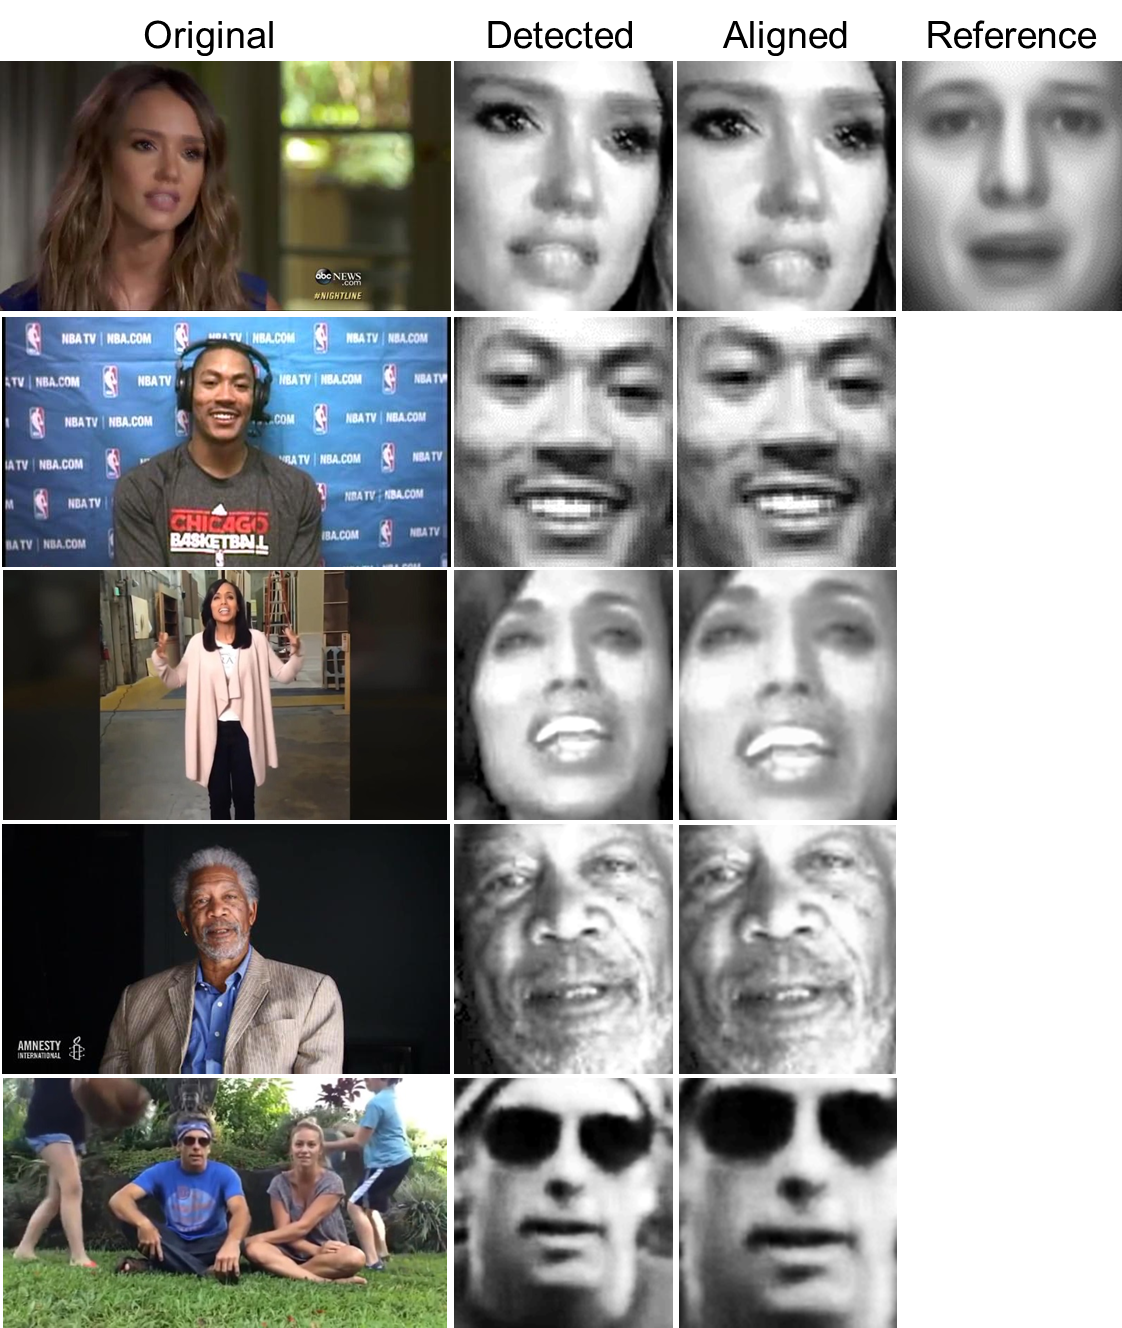
\includegraphics[width=.8\columnwidth]{fig/suppliment.png}
	\caption{Examples of face alignment results using SOFIT. By aligning with a canonical reference face, all pose rotations, translations, and scales are rectified. }
	\label{fig:suppliment}
\end{figure}



\subsection{Multi-frame Image Super-resolution}

\begin{figure}[t]
	\centering
		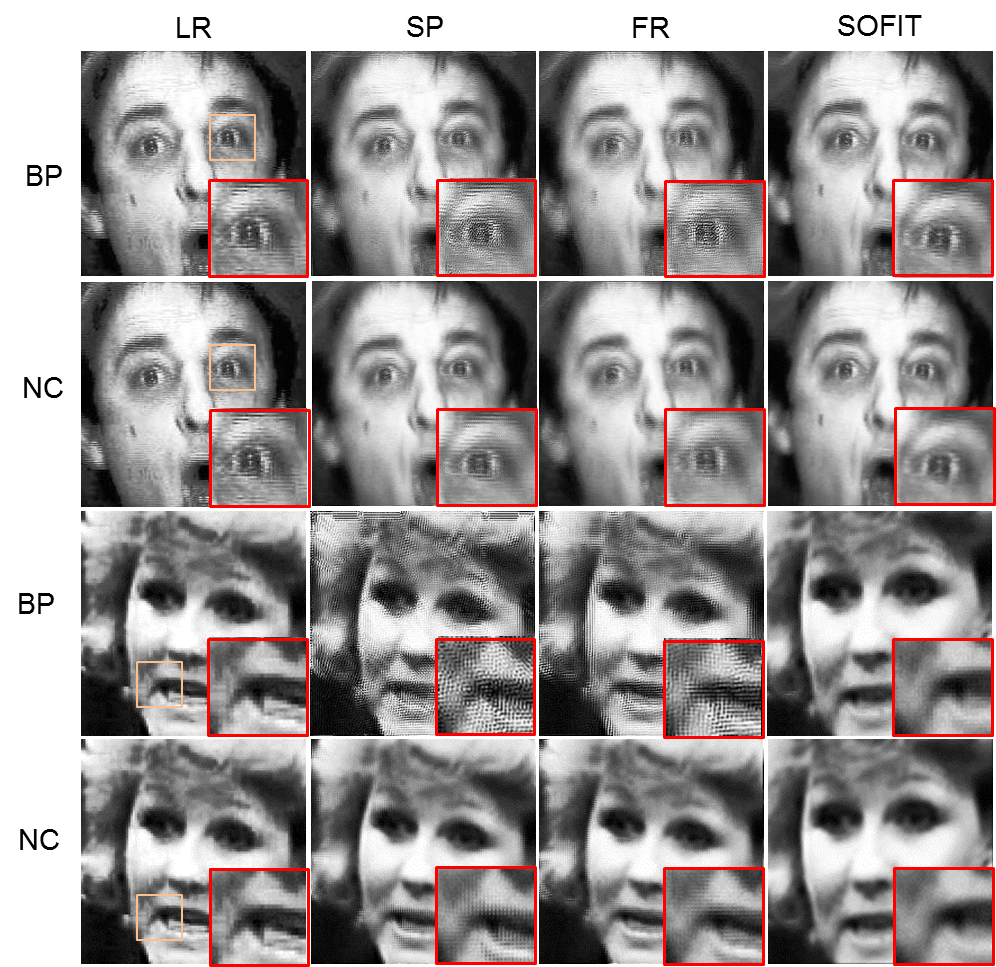
\includegraphics[width=\columnwidth]{fig/superResolution.png}
	\caption{The comparison of super-resolution results using different registration methods for 2 subjects. For each column from left to right: one of the LR inputs (enlarged by pixel replication), sub-pixel registration (SP)~\cite{Keren_CVPR88}, frequency domain based registration (FR)~\cite{Vandewalle06}, and the proposed registration method. We use two SR methods to reconstruct the high-resolution outputs: iterated back-projection (BP)~\cite{Irani91} and normalized convolution (NC)~\cite{Pham_06}. The red blocks show the magnified parts from the yellow blocks.}
	\label{fig:superResolution}
\end{figure}



In the imaging process, it is common to acquire images with low-resolution (LR) and/or certain artifacts such as blurriness, noise, \textit{etc}. Image super-resolution (SR) is the process of generating a high-resolution (HR) image from one or more LR inputs. In the past few decades, there has been extensive work on super-resolution methods. Based on the inputs, the SR algorithms can be classified in two categories: single-image based~\cite{Sun_CVPR08} and multi-image based methods~\cite{Irani91}. We apply SOFIT registration algorithm proposed in this paper to generate aligned images as inputs to different multi-image based SR methods. Here we compare our registration method with two other ones: frequency domain based method (FR)~\cite{Vandewalle06}, and registration using sub-pixel displacement (SP)~\cite{Keren_CVPR88}. These registration methods are then used in two SR methods: iterated back-projection (BP)~\cite{Irani91}, and normalized convolution based method (NC)~\cite{Pham_06}. Fig.~\ref{fig:superResolution} shows the visual comparison of some sample results using different registration methods in different SR algorithms.


\begin{figure}[t]
	\centering
		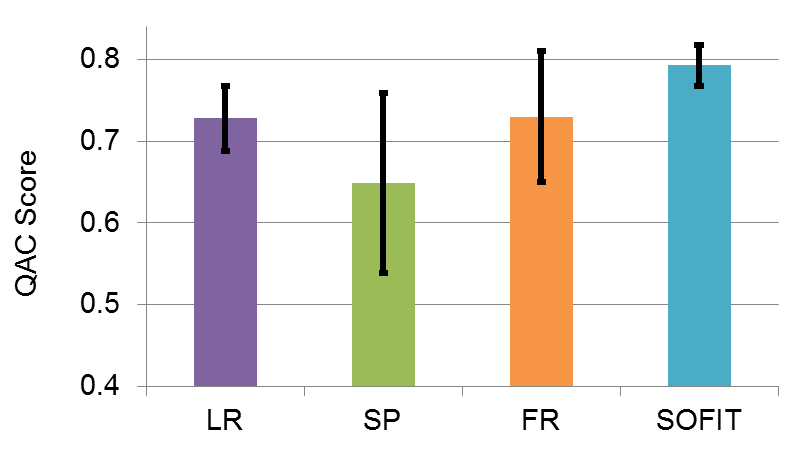
\includegraphics[width=.8\columnwidth]{fig/SR_quant.png}
	\caption{Image quality comparison between video-based super-resolution results and the proposed method, SOFIT. A recent non-reference image quality assessment method~\cite{Xue_CVPR13} is used. The higher the score, the better the estimated visual quality is. LR stands for low-resolution input images. SP denotes the super-resolved results using~\cite{Keren_CVPR88}. FR is the super-resolved results using~\cite{Vandewalle06}. SOFIT outperform other benchmarks and has less variance, indicated by the black line. }
	\label{fig:SR_quant}
\end{figure}


From Fig.~\ref{fig:superResolution} we can see that with our registration method, the SR results are significantly improved over the other SR methods in terms of visual quality. Despite the poor quality of the input frames, the results by our method are smooth with much fewer artifacts (\textit{e.g.}, noise and blockiness). The gain on the performance of SR directly comes from the accurate registration by the proposed method.. The output images by our methods are also well rectified which would be desirable for post-processing or subsequent recognition tasks. 




To quantitatively evaluate the image quality using our registration method, we compute a recently proposed non-reference image quality index, Quality-aware clustering (QAC)~\cite{Xue_CVPR13}, for output images using our method and the competing super-resolution methods. QAC is a general purpose blind image quality assessment method that has high correlation with human perception of image quality. Fig.~\ref{fig:SR_quant} lists the average image quality scores on 87 sequences from GEMEP-FERA database~\cite{FERA11}. Compared to the LR input and output using different registration methods, the output of SOFIT achieves the highest scores with the lowest standard deviation, which indicates better visual quality in terms of QAC image quality measure.



\subsection{Generic Object Registration}


\begin{figure*}[htbp]
	\centering
		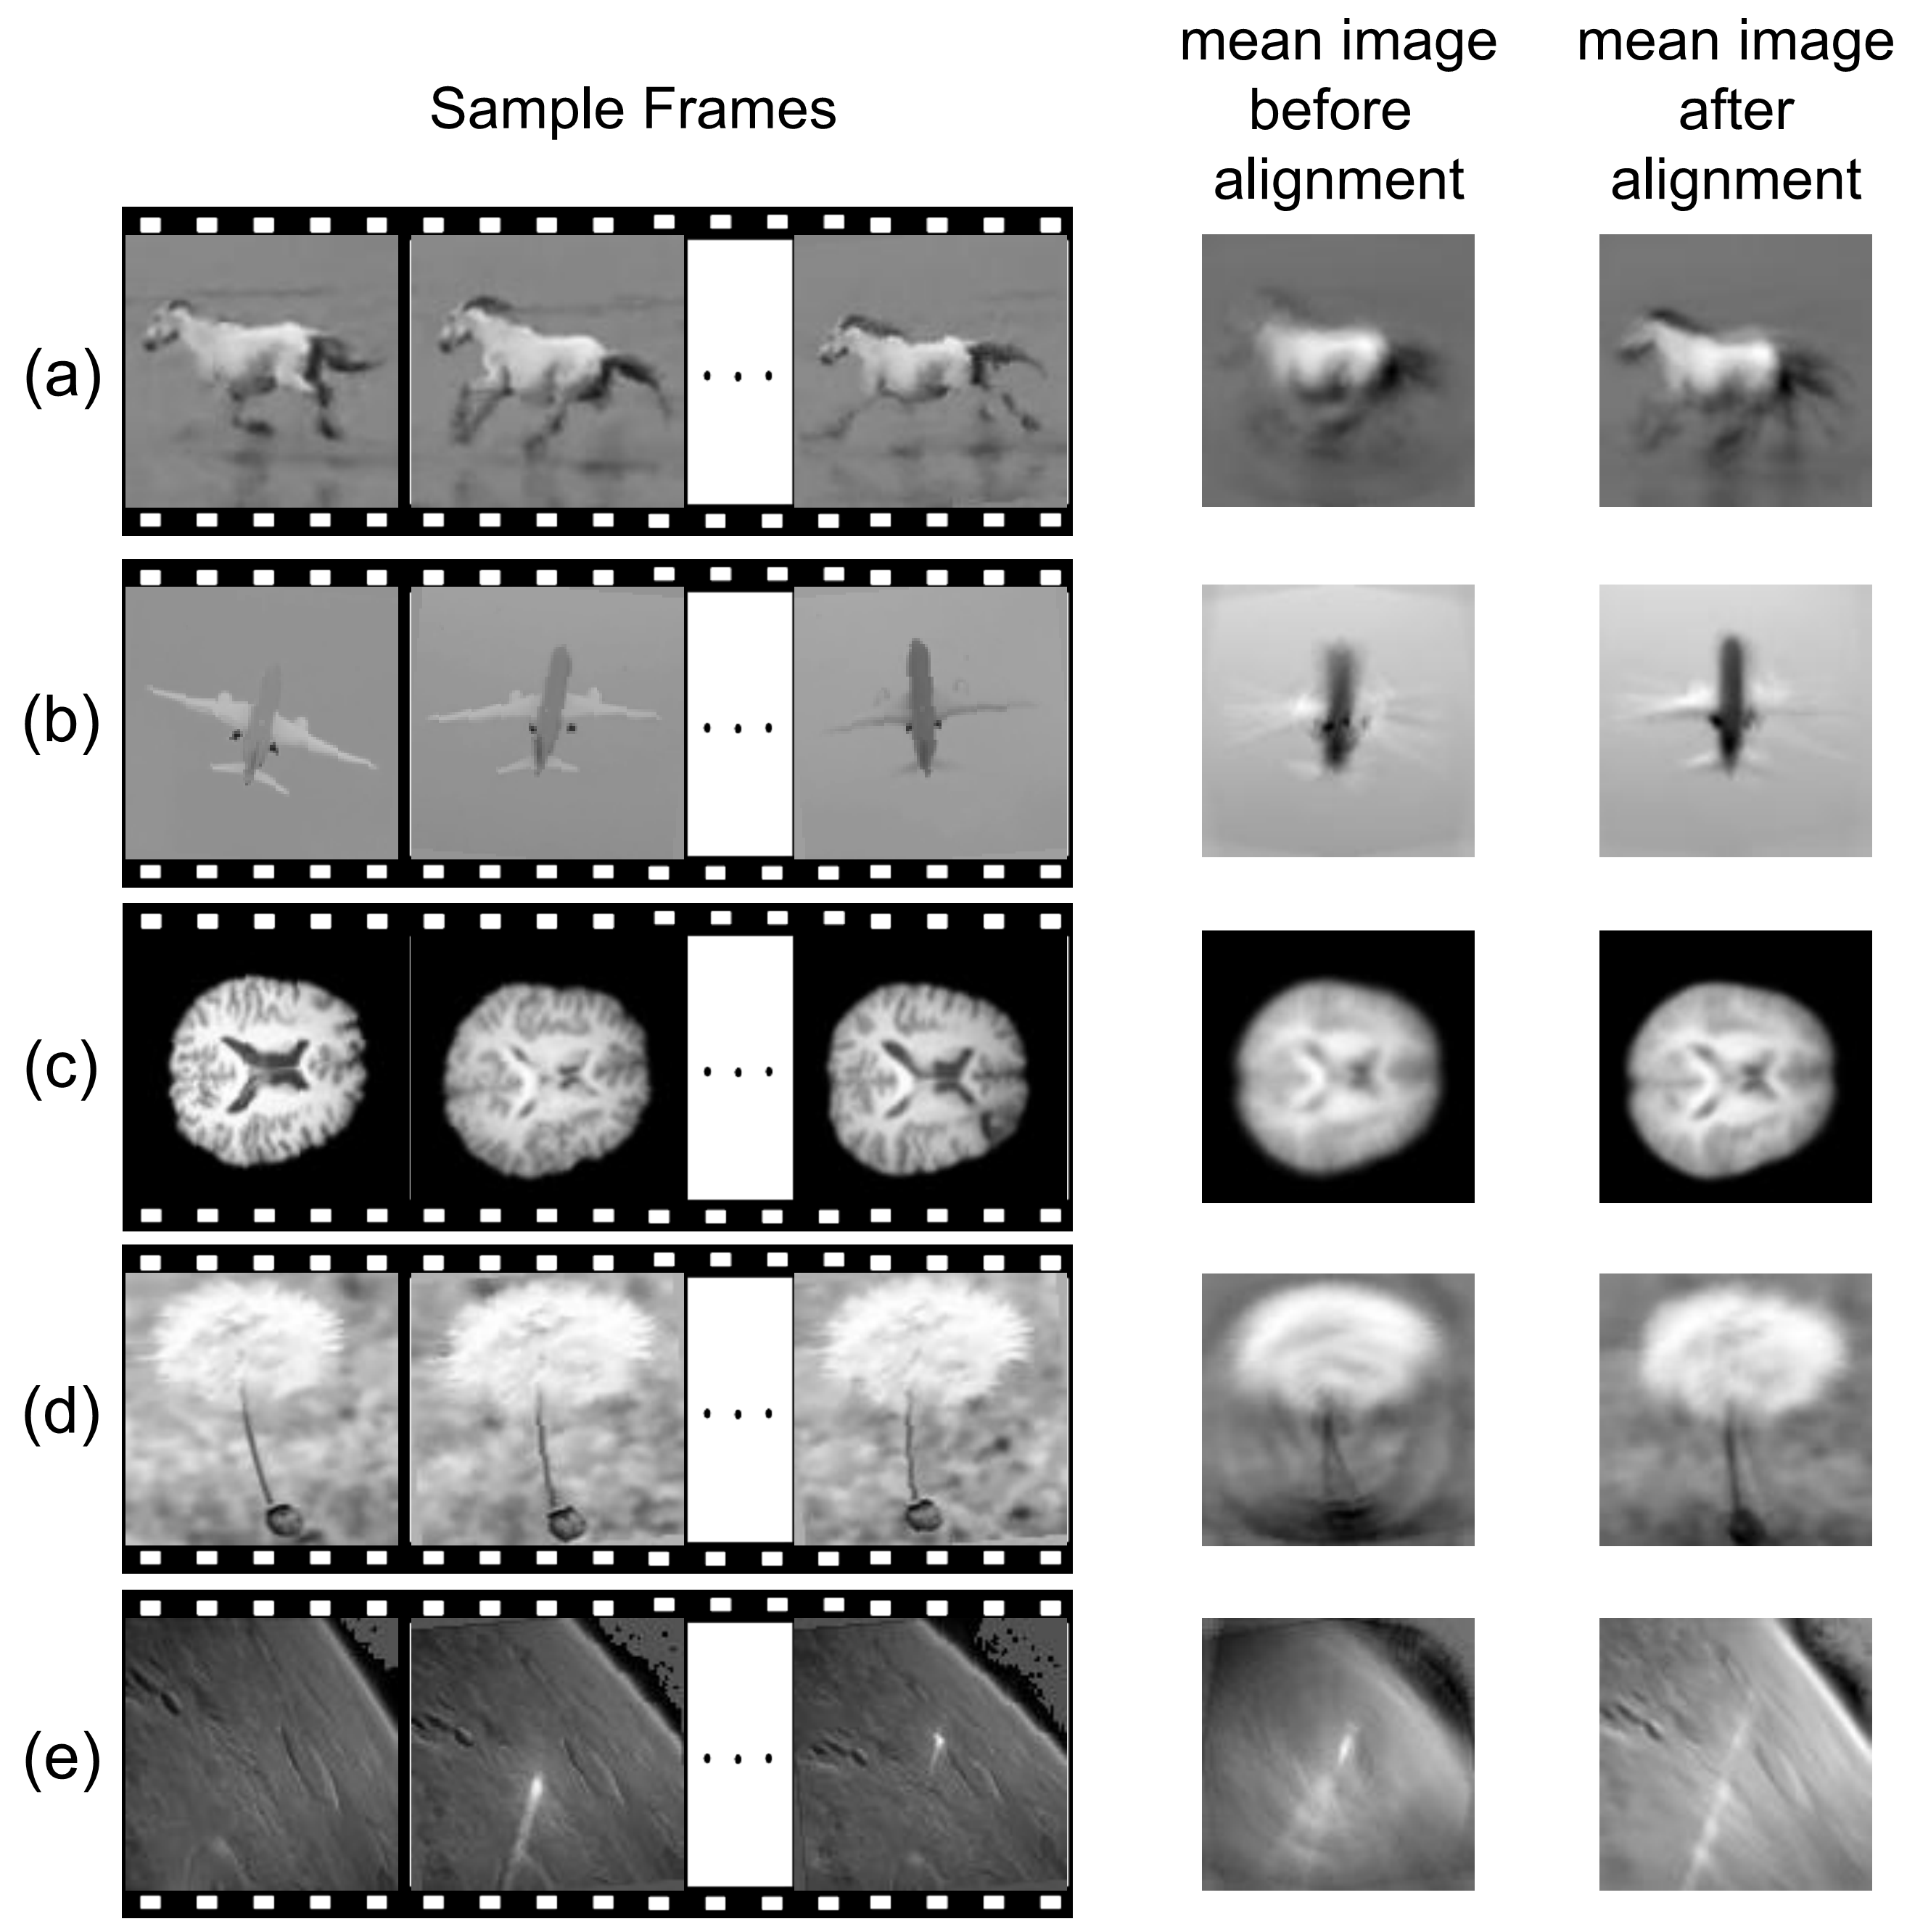
\includegraphics[width=.65\textwidth]{fig/object_ex.png}
	\caption{Sample registration results using SOFIT for generic objects in video, each row of which represents challenges in different aspects. The reference frame is randomly selected from each sequence and the average representations before/after SOFIT alignment are shown in the last two columns. The average between-frame optical flow length is computed to evaluate the smoothness of a sequence. It is observed that the average optical flow length becomes smaller after alignment, demonstrating an image sequence with smoother transition generated by our algorithm. (a) Non-rigid motion, mainly caused by the poses of a horse. (b) In-plane and out-of-plane rotation. (c) Appearance variation. This row contains Magnetic Resonance Imaging (MRI) samples from different individuals. Though it is not strictly video per se, the results show that our method is robust against intensity variations. (d) Cluttered background. (e) Outliers. While the camera is non-stationary, there is a rocket moving against the Mars. Since we explicitly model the dominant motion of the scene, outliers (such as the rocket) have little impact on the alignment results. The number below each image is the average between-frame optical flow length of an entire sequence; lower number indicates a smoother sequence.}
	\label{fig:object_ex}
\end{figure*}

In addition, we apply our method to other objects with challenges in various aspects, as shown in Fig.~\ref{fig:object_ex}. Each video contains approximately 50 frames of a detected object with compound motions. For each video, we randomly select one frame to be the reference as the input of our method. The visual registration results are shown in the last two columns of Fig.~\ref{fig:object_ex}, where the mean image results are sharper and reveals more local details. To quantitatively demonstrate that our algorithm generates image sequences with smoother transition, the $\ell_2$ norm of the between-frame optical flow is computed and then averaged across the entire sequence. It is essentially the average optical flow length of a sequence, reported below the corresponding mean image in Fig.~\ref{fig:object_ex}. It is observed that the average optical flow length is generally smaller, indicating a smoother sequence after our alignment algorithm.

\subsection{Limitations}
The proposed method assumes that the objects are already detected at similar scales. Such assumption holds in practice for some applications such as face analysis, which are indeed our main focus in this paper. Object detection in general is still a challenging topic. It still needs a great amount of effort to improve its performance even in predefined domains, such as face detection and pedestrian detection in the wild under low image resolution. For applications in which the detection itself is difficult or the object scale varies greatly, our method may fail to work.


\section{Conclusions\label{sec:conclusion}}

We developed a real-time video-alignment technique, SOFIT, to register objects with compound motion (\textit{i.e.} non-rigid surface motion accompanied by rigid body motion). We demonstrated its effectiveness in applications such as AU recognition and image super-resolution. This approach utilizes holistic dense flow-based information, and therefore, it is robust against detection error and noise. Minor out-of-plane rotation can also be corrected by employing structural correspondence from SIFT flow. More importantly, this method is able to generate temporally smooth registration results, which can improve the performance of various recognition and image super-resolution tasks.

%\section{Acknowledgements}
%
%This material is based upon work supported by the National Science Foundation under Grant No.
%0727129 and 0915270.
%The authors would like to thank Dr. Michel Valstar from the University of Nottingham, the organizer of FERA 2011 Challenge, for evaluating the AU testing results.

% Can use something like this to put references on a page
% by themselves when using endfloat and the captionsoff option.
\ifCLASSOPTIONcaptionsoff
  \newpage
\fi



% trigger a \newpage just before the given reference
% number - used to balance the columns on the last page
% adjust value as needed - may need to be readjusted if
% the document is modified later
%\IEEEtriggeratref{8}
% The "triggered" command can be changed if desired:
%\IEEEtriggercmd{\enlargethispage{-5in}}

% references section

% can use a bibliography generated by BibTeX as a .bbl file
% BibTeX documentation can be easily obtained at:
% http://www.ctan.org/tex-archive/biblio/bibtex/contrib/doc/
% The IEEEtran BibTeX style support page is at:
% http://www.michaelshell.org/tex/ieeetran/bibtex/
%\bibliographystyle{IEEEtran}
% argument is your BibTeX string definitions and bibliography database(s)
%\bibliography{IEEEabrv,../bib/paper}
%
% <OR> manually copy in the resultant .bbl file
% set second argument of \begin to the number of references
% (used to reserve space for the reference number labels box)
\bibliographystyle{IEEEtran}
\bibliography{SOFA}


\begin{IEEEbiography}[{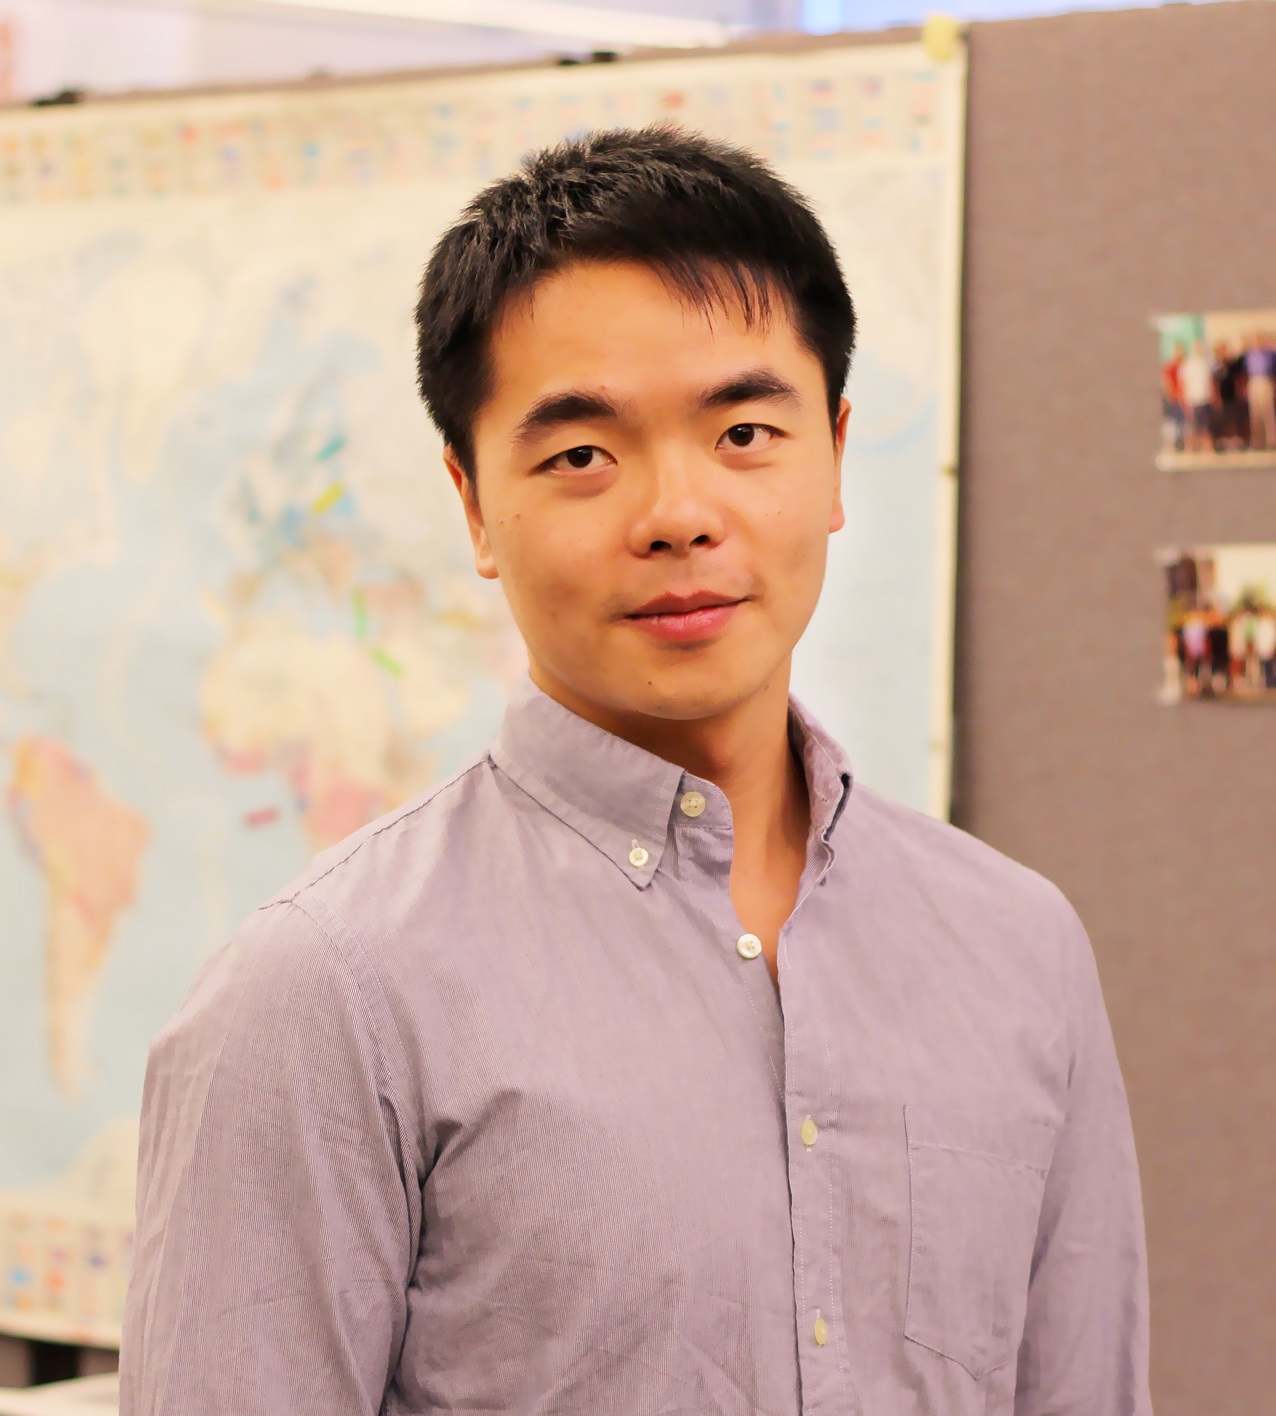
\includegraphics[width=1in,height=1.25in,clip,keepaspectratio]{pic/songfan.jpg}}]{Songfan Yang}
(S'10-M'14) received the B.S. degree in Electrical Engineering from Sichuan University, Chengdu, China, in 2009 and the M.S. and Ph.D. degree in Electrical Engineering from University of California, Riverside. He is currently an Associate Professor of College of Electronics and Information Engineering at Sichuan University. His research interests include computer vision, pattern recognition, and affective computing. He holds the Best Entry Award of the FG 2011 Facial Expression Recognition and Analysis emotion challenge (FERA) competition.
\end{IEEEbiography}

\begin{IEEEbiography}[{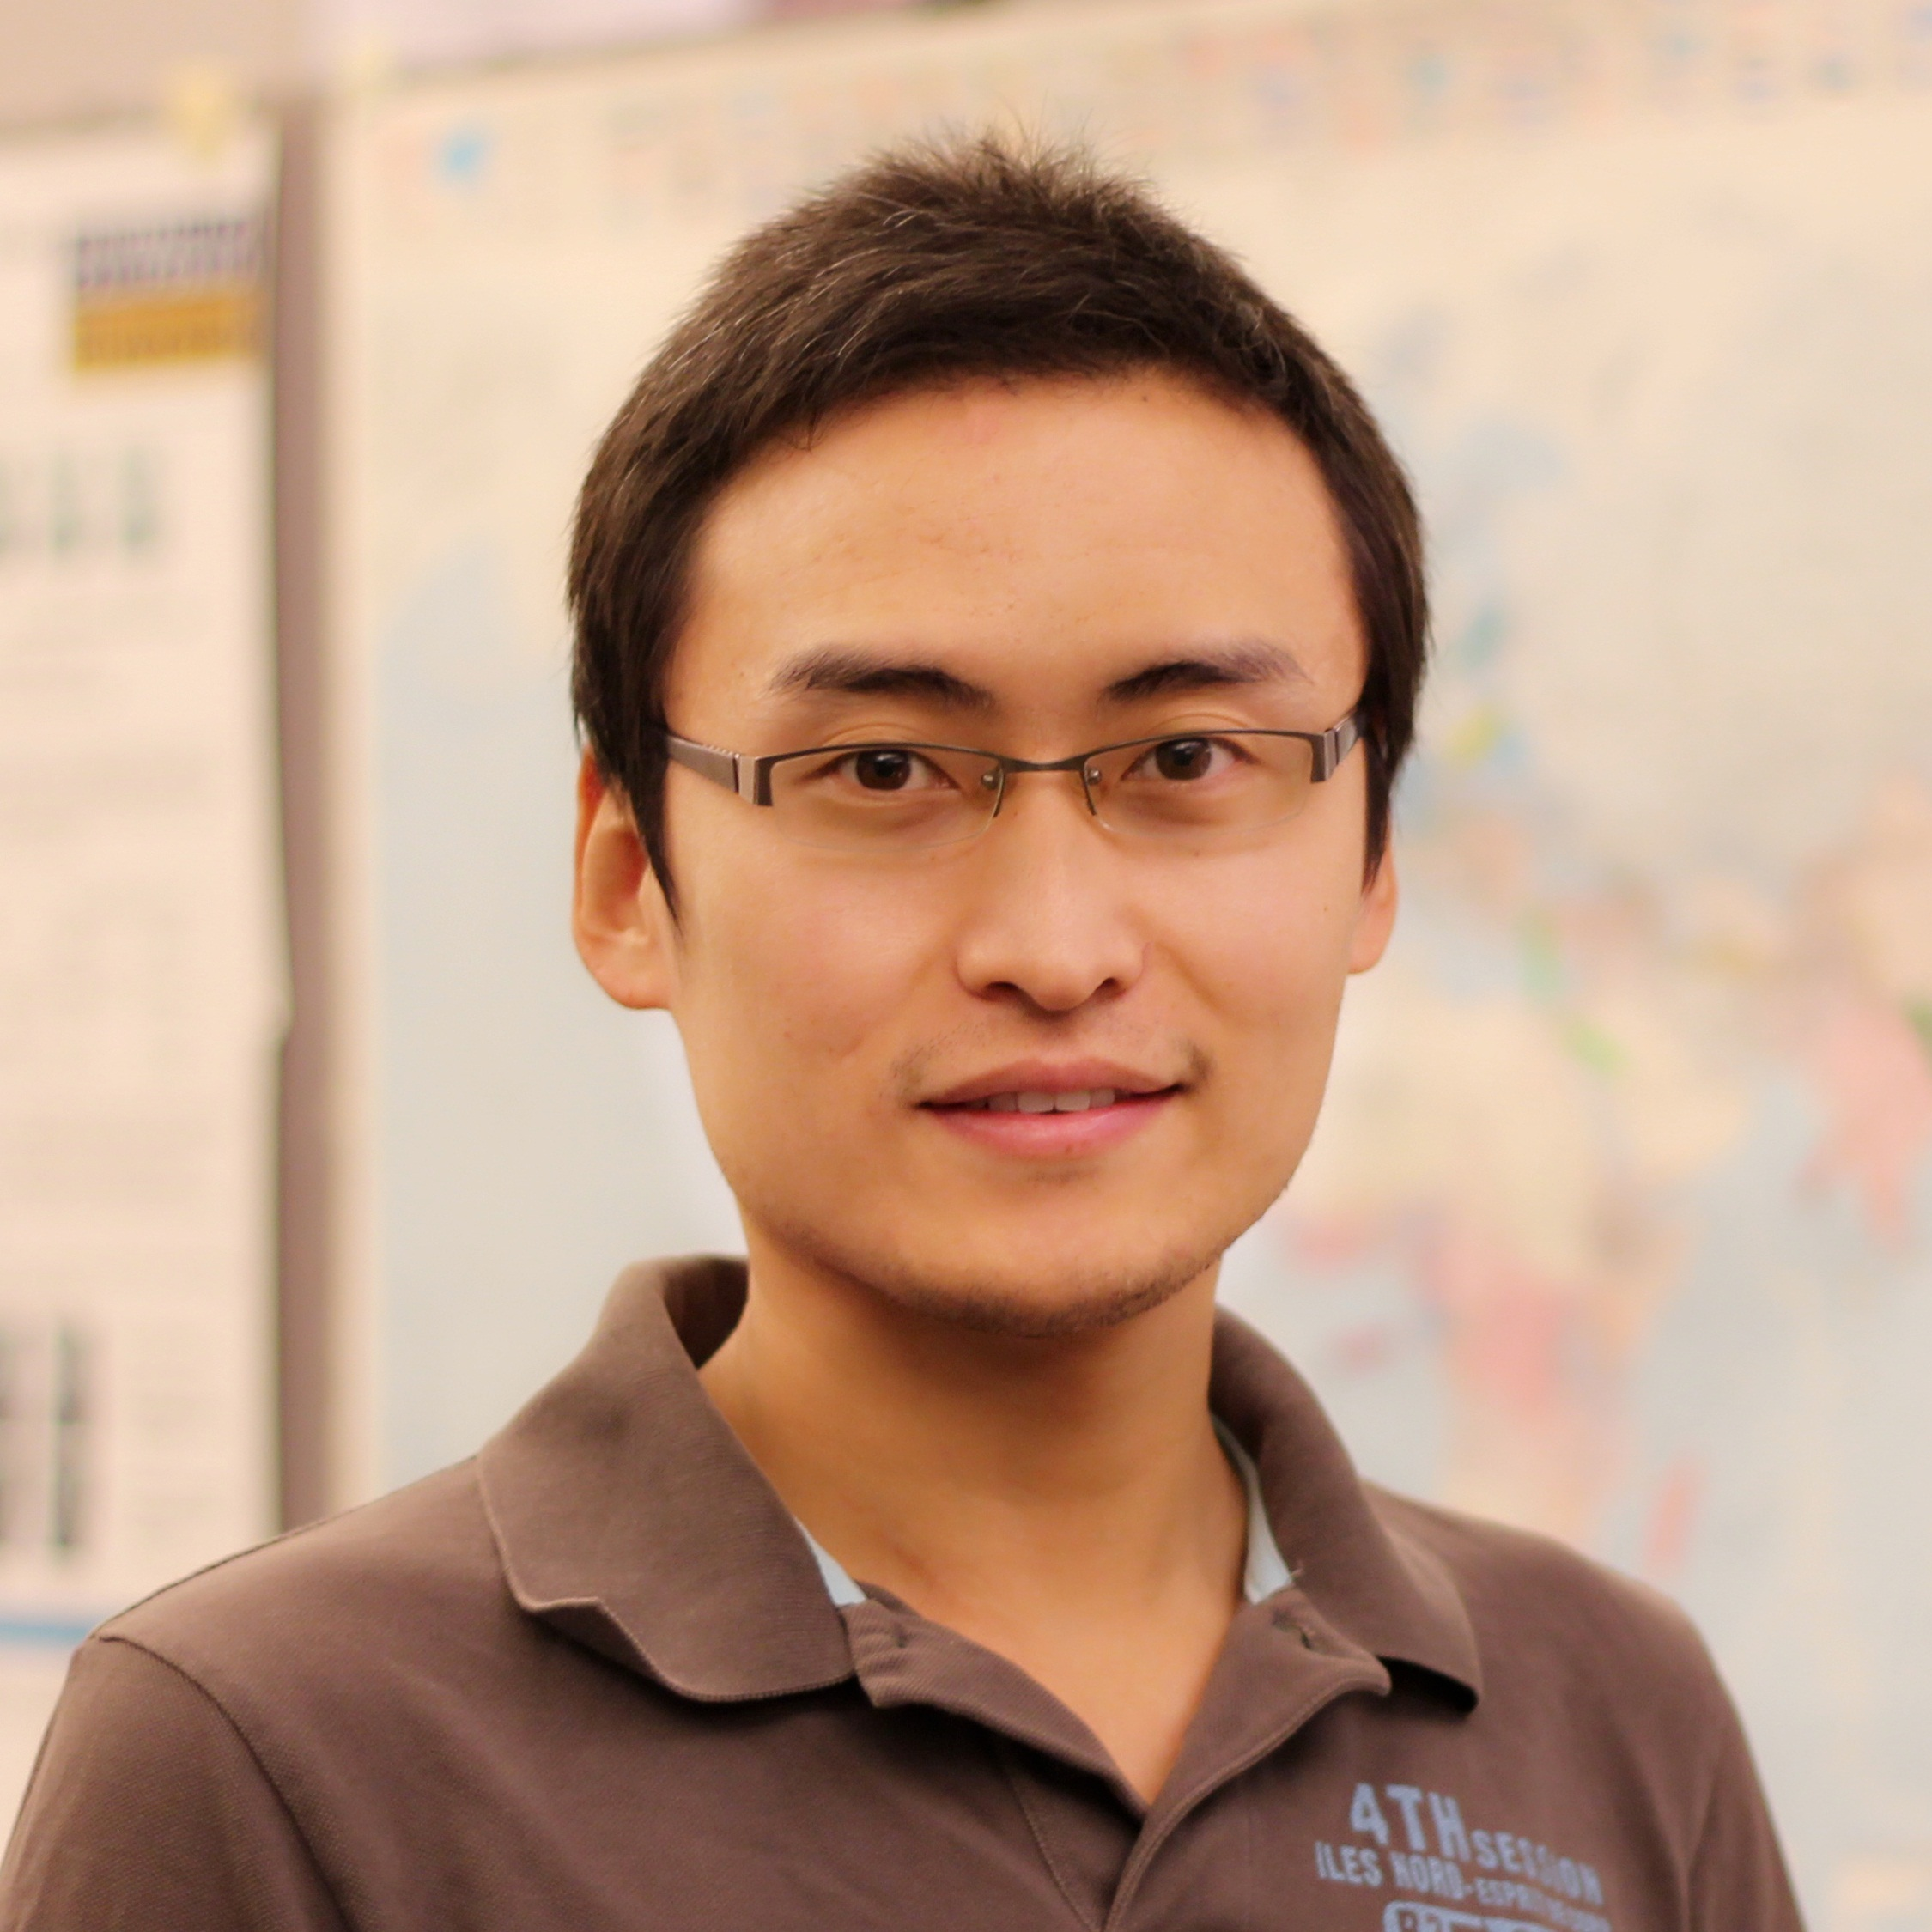
\includegraphics[width=1in,height=1.25in,clip,keepaspectratio]{pic/Lean.jpg}}]{Le An} received the B.Eng. degree in telecommunications engineering from Zhejiang University in China in 2006, the MSc degree in electrical engineering from Eindhoven University of Technology in Netherlands in 2008, and the PhD degree in electrical engineering from University of California, Riverside in USA in 2014. He is currently a postdoctoral research associate at University of North Carolina at Chapel Hill, USA.  
His research interests include image processing, computer vision, pattern recognition, and machine learning. He received the best paper award from the 2013 IEEE International Conference on Advanced Video and Signal-Based Surveillance (AVSS).
\end{IEEEbiography}

\begin{IEEEbiography}[{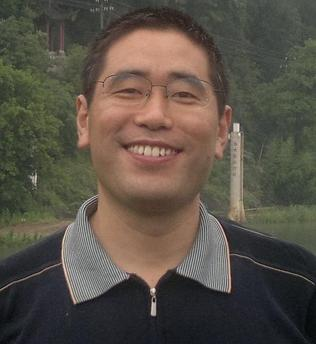
\includegraphics[width=1in,height=1.25in,clip,keepaspectratio]{pic/yiguang.jpg}}]{Yiguang Liu} received the M.S. degree from Peking University, Beijing, China, in 1998, and the Ph.D. degree from Sichuan University, Chengdu, China, in 2004. He was a Research Fellow, Visiting Professor, and Senior Research Scholar with the National University of Singapore, Singapore, Imperial College London, London, U.K., and Michigan State University, East Lansing, MI, USA, respectively. He was chosen into the program for new century excellent talents of MOE in 2008, and chosen as a Scientific and Technical Leader in Sichuan Province in 2010. He is currently the Director of the Vision and Image Processing Laboratory and a Professor with the School of Computer Science, Sichuan University. He has co-authored over 100 international journal and conference papers, and a chapter of the book entitled Computational Intelligence and Its Applications (H.K.Lam). His current research interests include computer vision and image processing, pattern recognition, and computational intelligence. Dr. Liu is a Reviewer of Mathematical Reviews of the American Mathematical Society.
\end{IEEEbiography}


\begin{IEEEbiography}[{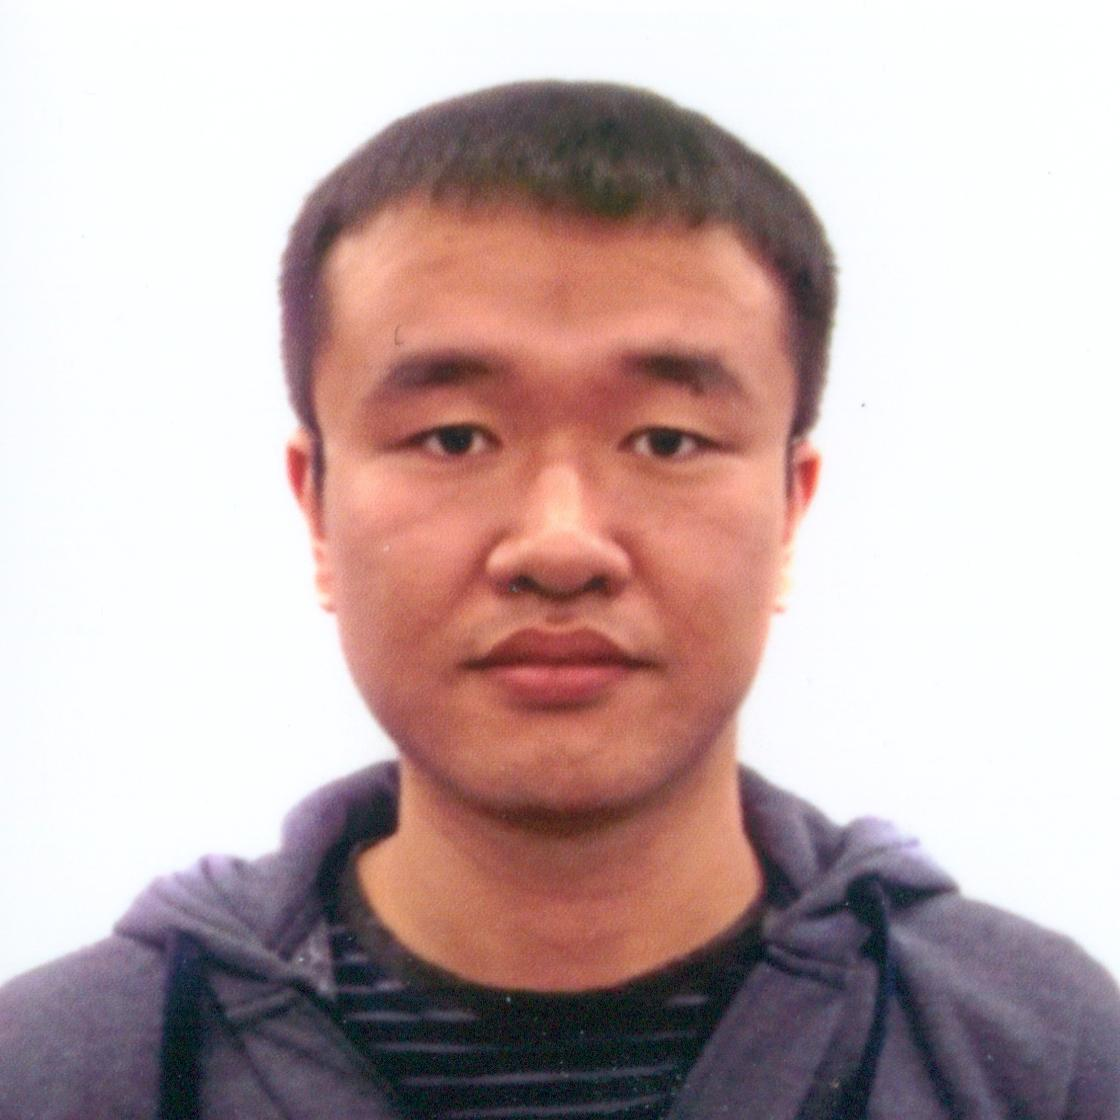
\includegraphics[width=1in,height=1.25in,clip,keepaspectratio]{pic/mingyang.jpg}}]{Mingyang Li} received B.Eng. degree in Automation Engineering from University of Electronic Science and Technology of China, Chengdu, China, in 2009, and Ph.D. degree in
Electrical Engineering from University of California, Riverside, in 2014. He is currently working as a research software engineer at Google Inc. His research interest lies primarily in the areas of robotics and computer vision. In particular, his research focuses sensor fusion, vision-aided inertial navigation, and multiple-view geometry in computer vision. 

\end{IEEEbiography}


\begin{IEEEbiography}[{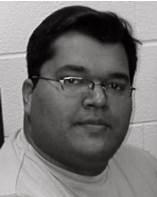
\includegraphics[width=1in,height=1.25in,clip,keepaspectratio]{pic/ninad}}]{Ninad Thakoor} 
(S'04-M'10) received the BE degree in electronics and telecommunication engineering from the University of Mumbai, India, in 2001, and the MS and PhD degrees in electrical engineering from the University of Texas at Arlington, in 2004 and 2009, respectively. He is with Center for Research in Intelligent System at University of California at Riverside as a postdoctoral researcher.

His current research interests include vehicle recognition, stereo disparity segmentation, and structure-and-motion segmentation.
\end{IEEEbiography}



\begin{IEEEbiography}[{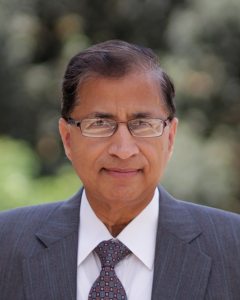
\includegraphics[width=1in,height=1.25in,clip,keepaspectratio]{pic/bhanu}}]{Bir Bhanu}
(S'72-M'82-SM'87-F'95) received the S.M. and E.E. degrees in Electrical Engineering and Computer Science from the Massachusetts Institute of Technology, Cambridge, MA, the Ph.D. degree in Electrical Engineering, from the Image Processing Institute at University of Southern California and the M.B.A. degree from the University of California, Irvine. He is the Distinguished Professor of Electrical Engineering and Cooperative Professor of Computer Science and Engineering, Mechanical Engineering and Bioengineering, and the Director of the Center for Research in Intelligent Systems (CRIS) and the Visualization and Intelligent Systems Laboratory (VISLab) at the University of California, Riverside (UCR). In addition, he serves as the director of NSF IGERT on Video Bioinformatics at UCR. Dr. Bhanu has been the Principal Investigator of various programs for NSF, DARPA, NASA, AFOSR, ONR, ARO, and other agencies and industries in the areas of video networks, video understanding, video bioinformatics, learning and vision, image understanding, pattern recognition, target recognition, biometrics, autonomous navigation, image databases, and machine-vision applications. He has published seven coauthored and three edited books. He is the holder of 18 (3 pending) patents. He has published more than 500 reviewed technical publications, including over 140 journal papers and 44 book chapters. His current research interests are Computer Vision, Pattern Recognition and Data Mining, Machine Learning, Artificial Intelligence, Image Processing, Image and Video Database, Graphics and Visualization, Robotics, Human-Computer Interactions, Biological, Medical, Military and Intelligence applications. He is Fellow of IEEE, AAAS, IAPR, and SPIE.
\end{IEEEbiography}


% if you will not have a photo at all:


% You can push biographies down or up by placing
% a \vfill before or after them. The appropriate
% use of \vfill depends on what kind of text is
% on the last page and whether or not the columns
% are being equalized.

%\vfill

% Can be used to pull up biographies so that the bottom of the last one
% is flush with the other column.
%\enlargethispage{-5in}



% that's all folks
\end{document}
